%!TEX program = xelatex
% ============================================================
%  机器学习基础 · 讲义  ——  奇异值分解
%  编译方式：xelatex 两次
% ============================================================
\documentclass[UTF8, 11pt, a4paper, fontset=windows]{ctexart}

% ---------- 字体与数学 ----------
\usepackage{amsmath}
\usepackage{unicode-math}
\setmathfont{TeX Gyre Termes Math}
\setmathfont{TeX Gyre Termes Math}[version=bold, FakeBold=1.8]
\setmainfont{TeX Gyre Termes}
\setmonofont{Consolas}[Scale=0.92]

% ---------- 版面 ----------
\usepackage[top=2.7cm, bottom=2.6cm, left=2.5cm, right=2.5cm,
            headheight=15pt, headsep=0.7cm, footskip=1.1cm]{geometry}
\linespread{1.42}
\setlength{\parskip}{0.32em}
\setlength{\parindent}{2em}
\emergencystretch=2.5em

% ---------- 颜色 ----------
\usepackage{xcolor}
\definecolor{navy}{RGB}{11,44,77}        % 海军深蓝（主色）
\definecolor{navydeep}{RGB}{6,26,47}     % 更深的蓝
\definecolor{navymid}{RGB}{31,77,124}    % 中间蓝
\definecolor{navypale}{RGB}{233,239,246} % 极浅蓝
\definecolor{gold}{RGB}{170,136,84}      % 暗金（点缀）
\definecolor{ink}{RGB}{26,30,36}         % 正文墨色
\definecolor{warnc}{RGB}{134,58,52}      % 警示暗红

\color{ink}

% ---------- 表格、列表 ----------
\usepackage{booktabs}
\usepackage{float}
\usepackage{array}
\usepackage{enumitem}
\setlist[itemize]{leftmargin=1.9em, itemsep=2.5pt, topsep=5pt, parsep=0pt, label=\textcolor{navy}{\textbullet}}
\setlist[enumerate]{leftmargin=2.1em, itemsep=3pt, topsep=5pt, parsep=0pt,
                    label=\textcolor{navy}{\bfseries\arabic*.}}

% ---------- 图形 ----------
\usepackage{tikz}
\usetikzlibrary{arrows.meta, positioning, calc, patterns, decorations.pathreplacing}
\usepackage[most]{tcolorbox}

% ---------- 页眉页脚 ----------
\usepackage{fancyhdr}
\pagestyle{fancy}
\fancyhf{}
\fancyhead[L]{\small\sffamily\color{navy!65}机器学习基础\,\textperiodcentered\,讲义}
\fancyhead[R]{\small\sffamily\color{navy!65}\nouppercase{\leftmark}}
\fancyfoot[C]{\small\color{navy!55}\thepage}
\renewcommand{\headrulewidth}{0.6pt}
\renewcommand{\headrule}{\hbox to\headwidth{\color{navy!35}\leaders\hrule height \headrulewidth\hfill}}
\fancypagestyle{plain}{\fancyhf{}\fancyfoot[C]{\small\color{navy!55}\thepage}%
  \renewcommand{\headrulewidth}{0pt}}

% ---------- 标题样式 ----------
\usepackage{titlesec}
\titleformat{\section}[hang]
  {\normalfont\Large\sffamily\bfseries\color{navy}}
  {\raisebox{-0.1em}{\colorbox{navy}{\makebox[1.85em][c]{\color{white}\normalsize\sffamily\bfseries\thesection}}}\hspace{0.65em}}
  {0pt}{}
  [\vspace{-0.32em}{\color{navy!22}\rule{\linewidth}{0.9pt}}]
\titlespacing*{\section}{0pt}{2.1em plus 0.4em minus 0.2em}{1.0em plus 0.3em}

\titleformat{\subsection}[hang]
  {\normalfont\large\sffamily\bfseries\color{navy!92}}
  {\textcolor{gold}{\rule[0.30em]{0.36em}{0.36em}}\hspace{0.42em}\thesubsection}
  {0.55em}{}
\titlespacing*{\subsection}{0pt}{1.5em plus 0.3em minus 0.2em}{0.75em plus 0.2em}

\titleformat{\subsubsection}[hang]
  {\normalfont\normalsize\sffamily\bfseries\color{navy!85}}
  {\thesubsubsection}{0.5em}{}
\titlespacing*{\subsubsection}{0pt}{1.1em plus 0.2em}{0.5em}

\titleformat{name=\section,numberless}[hang]
  {\normalfont\Large\sffamily\bfseries\color{navy}}
  {}{0pt}{}
  [\vspace{-0.32em}{\color{navy!22}\rule{\linewidth}{0.9pt}}]

\renewcommand{\contentsname}{\sffamily 目\quad 录}
\setcounter{tocdepth}{2}

% ---------- 定理环境 ----------
\usepackage{amsthm}
\newtheoremstyle{cnthm}
  {0.3em}{0.3em}{\normalfont}{0pt}
  {\sffamily\bfseries\color{navy}}{}{\newline}
  {\thmname{#1}\thmnumber{ #2}\thmnote{\ \textnormal{\sffamily（#3）}}}
\newtheoremstyle{cndef}
  {0.3em}{0.3em}{\normalfont}{0pt}
  {\sffamily\bfseries\color{navymid}}{}{\newline}
  {\thmname{#1}\thmnumber{ #2}\thmnote{\ \textnormal{\sffamily（#3）}}}

\theoremstyle{cnthm}
\newtheorem{thm}{定理}[section]
\newtheorem{lemma}[thm]{引理}
\newtheorem{prop}[thm]{命题}
\newtheorem{cor}[thm]{推论}

\theoremstyle{cndef}
\newtheorem{defn}{定义}[section]
\newtheorem{exam}[defn]{例}
\newtheorem{rem}[defn]{注}

% 定理盒：白底 + 深蓝左线
\tcolorboxenvironment{thm}{
  enhanced, colback=white, colframe=white, boxrule=0pt,
  borderline west={2.6pt}{0pt}{navy},
  arc=0pt, outer arc=0pt, left=12pt, right=4pt, top=6pt, bottom=6pt,
  before skip=11pt, after skip=11pt}
\tcolorboxenvironment{lemma}{
  enhanced, colback=white, colframe=white, boxrule=0pt,
  borderline west={2.6pt}{0pt}{navy!75},
  arc=0pt, outer arc=0pt, left=12pt, right=4pt, top=6pt, bottom=6pt,
  before skip=11pt, after skip=11pt}
\tcolorboxenvironment{prop}{
  enhanced, colback=white, colframe=white, boxrule=0pt,
  borderline west={2.6pt}{0pt}{navy!75},
  arc=0pt, outer arc=0pt, left=12pt, right=4pt, top=6pt, bottom=6pt,
  before skip=11pt, after skip=11pt}
\tcolorboxenvironment{cor}{
  enhanced, colback=white, colframe=white, boxrule=0pt,
  borderline west={2.6pt}{0pt}{navy!55},
  arc=0pt, outer arc=0pt, left=12pt, right=4pt, top=6pt, bottom=6pt,
  before skip=11pt, after skip=11pt}
% 定义盒：浅蓝底
\tcolorboxenvironment{defn}{
  enhanced, colback=navypale, colframe=navypale, boxrule=0pt,
  borderline west={2.6pt}{0pt}{navymid},
  arc=0pt, outer arc=0pt, left=12pt, right=9pt, top=7pt, bottom=7pt,
  before skip=11pt, after skip=11pt}
\tcolorboxenvironment{exam}{
  enhanced, colback=navypale!45!white, colframe=navypale!45!white, boxrule=0pt,
  borderline west={2.6pt}{0pt}{gold!80!black},
  arc=0pt, outer arc=0pt, left=12pt, right=9pt, top=7pt, bottom=7pt,
  before skip=11pt, after skip=11pt}
\tcolorboxenvironment{rem}{
  enhanced, colback=white, colframe=white, boxrule=0pt,
  borderline west={1.6pt}{0pt}{navy!30},
  arc=0pt, outer arc=0pt, left=12pt, right=4pt, top=5pt, bottom=5pt,
  before skip=10pt, after skip=10pt}

% 提示类盒子
\newtcolorbox{insight}[1][直觉]{
  enhanced, breakable, colback=gold!6!white, colframe=gold!6!white, boxrule=0pt,
  borderline west={2.4pt}{0pt}{gold},
  arc=0pt, outer arc=0pt, left=12pt, right=9pt, top=6pt, bottom=6pt,
  before skip=11pt, after skip=11pt,
  fonttitle=\sffamily\bfseries\small, coltitle=gold!55!black,
  attach title to upper={\quad}, title={#1}}
\newtcolorbox{warnbox}[1][易错点]{
  enhanced, breakable, colback=warnc!5!white, colframe=warnc!5!white, boxrule=0pt,
  borderline west={2.4pt}{0pt}{warnc},
  arc=0pt, outer arc=0pt, left=12pt, right=9pt, top=6pt, bottom=6pt,
  before skip=11pt, after skip=11pt,
  fonttitle=\sffamily\bfseries\small, coltitle=warnc,
  attach title to upper={\quad}, title={#1}}
\newtcolorbox{keybox}[1][要点]{
  enhanced, breakable, colback=navy, colframe=navy, boxrule=0pt,
  arc=1pt, outer arc=1pt, left=13pt, right=11pt, top=8pt, bottom=8pt,
  before skip=12pt, after skip=12pt, coltext=white,
  fonttitle=\sffamily\bfseries\small, coltitle=gold,
  attach title to upper={\quad}, title={#1}}

% ---------- 代码 ----------
\usepackage{listings}
\lstset{
  basicstyle=\ttfamily\footnotesize,
  keywordstyle=\color{navymid}\bfseries,
  commentstyle=\color{navy!45}\itshape,
  stringstyle=\color{gold!70!black},
  numbers=left, numberstyle=\tiny\color{navy!45}, numbersep=9pt,
  frame=leftline, framerule=2.4pt, rulecolor=\color{navy!65},
  backgroundcolor=\color{navypale!55!white},
  xleftmargin=20pt, xrightmargin=2pt,
  aboveskip=11pt, belowskip=11pt,
  showstringspaces=false, breaklines=true, columns=fullflexible, keepspaces=true,
  captionpos=b
}

% ---------- 超链接 ----------
\usepackage[colorlinks=true, linkcolor=navy, urlcolor=navymid, citecolor=navy,
            bookmarksnumbered=true, bookmarksopen=true]{hyperref}
\hypersetup{pdftitle={奇异值分解：从几何直觉到低秩近似},
            pdfauthor={小算},
            pdfsubject={机器学习基础讲义}}

% ---------- 常用宏 ----------
\newcommand{\inforow}[2]{%
  \noindent
  \begin{minipage}[t]{2.6cm}\sffamily\bfseries\color{navy}#1\end{minipage}%
  \hspace{0.25cm}%
  \begin{minipage}[t]{11.15cm}\setlength{\parindent}{0pt}\small #2\end{minipage}%
  \par\vspace{0.5em}}
\newcommand{\T}{^{\mathrm{T}}}
\newcommand{\R}{\mathbb{R}}
\newcommand{\nrm}[1]{\lVert #1 \rVert}
\newcommand{\abs}[1]{\lvert #1 \rvert}
\newcommand{\ip}[2]{\langle #1,\, #2\rangle}
\DeclareMathOperator{\rank}{rank}
\DeclareMathOperator{\tr}{tr}
\DeclareMathOperator{\diag}{diag}
\DeclareMathOperator{\Span}{span}
\DeclareMathOperator{\Null}{null}
\DeclareMathOperator{\Col}{col}
\DeclareMathOperator{\Row}{row}
\DeclareMathOperator*{\argmin}{arg\,min}
\newcommand{\bu}{\symbfit{u}}
\newcommand{\vct}{\symbfit{v}}
\newcommand{\x}{\symbfit{x}}
\newcommand{\y}{\symbfit{y}}
\newcommand{\bb}{\symbfit{b}}
\newcommand{\vv}{\symbfit{v}}

\begin{document}

% ============================================================
%  封面
% ============================================================
\begin{titlepage}
\thispagestyle{empty}
\begin{tikzpicture}[remember picture, overlay]
  \fill[navy] (current page.north west) rectangle ([yshift=-12.05cm]current page.north east);
  \fill[gold] ([yshift=-12.05cm]current page.north west) rectangle ([yshift=-12.12cm]current page.north east);
  \node[white, opacity=0.05, font=\fontsize{200}{200}\selectfont\bfseries]
       at ([xshift=-4.2cm, yshift=-7.9cm]current page.north east) {$\Sigma$};
\end{tikzpicture}%

\vspace*{1.05cm}
{\color{white!58!navy}\sffamily\large 机器学习基础\,\textperiodcentered\,讲义系列}

\vspace{1.0cm}
{\color{white}\sffamily\bfseries\fontsize{44}{48}\selectfont 奇异值分解}

\vspace{0.72cm}
{\color{white!82!navy}\sffamily\large 从几何直觉到低秩近似}

\vspace{0.62cm}
{\color{gold}\rule{3.0cm}{1.1pt}}

\vspace{0.52cm}

\vspace*{1.1cm}

\noindent{\color{navy!35}\rule{\linewidth}{0.6pt}}\par\vspace{0.55em}
\noindent{\color{navy!35}\rule{\linewidth}{0.6pt}}

\vspace{0.9cm}

\noindent
\begin{minipage}{\textwidth}
{\sffamily\bfseries\color{navy}内容提要}\quad
{\small
奇异值分解（SVD）把任意一个矩阵拆成“旋转—拉伸—旋转”三步，把一个看似只能处理方阵的工具，推广到了所有矩阵。本讲义从单位圆的形变讲起，逐步给出 SVD 的定义、存在性证明、基本性质与低秩逼近的 Eckart--Young 定理，并把它与最小二乘、主成分分析、图像压缩、推荐系统联系起来。全文的数值例子都可以手工验算，代码示例基于 NumPy。}
\end{minipage}

\vfill

\noindent

\end{titlepage}

% ============================================================
%  目录
% ============================================================
\pagenumbering{roman}
\setcounter{page}{1}
\pagestyle{plain}
\tableofcontents
\clearpage
\pagestyle{fancy}

\pagenumbering{arabic}
\setcounter{page}{1}

% ============================================================
\section{导读：为什么是奇异值分解}
% ============================================================

如果在一门机器学习课里只允许你记住一种矩阵分解，那应该就是奇异值分解（Singular
Value Decomposition，简称 SVD）。它几乎出现在所有需要“从大矩阵里提取主要结构”的
地方：图像压缩、推荐系统、数据降维、文本主题分析、系统辨识、网络嵌入。更重要的是，
它把线性代数里几个看似分散的概念——秩、范数、投影、最小二乘、条件数——串成了一条线。

本节先不谈定义，而是从三个具体问题出发，说明这些问题为什么最后都会指向同一个答案。

\subsection{三个看似无关的问题}

\paragraph{问题一：能不能用更少的数字存下一张照片？}
一张 $512\times 512$ 的灰度照片，本质上是 $512\times 512=262144$ 个灰度值。若每个
值用 1 字节存储，需要 256\,KB。可是照片里有大片平滑的天空、重复的砖墙纹理，真正
“变化”的部分远少于像素个数。我们能不能只用两三万个数字把它存下来，而肉眼几乎看不出
差别？

\paragraph{问题二：能不能猜出一个用户会给某部电影打几分？}
一个视频网站有一百万用户、五万部电影，评分矩阵有 $5\times 10^{10}$ 个格子，而实际
存在的评分不到 $1\%$。剩下的 $99\%$ 是空的。如何从这 $1\%$ 里推断出其余的评分，从而
做推荐？

\paragraph{问题三：能不能把 100 维的数据画在纸上？}
每个样本有 100 个特征，而人眼只能看二维平面。我们希望找两个方向，把数据投影上去，
既让点尽量散开，又尽量保留原来样本之间的远近关系。

这三个问题表面上属于图像处理、推荐系统、数据可视化三个不同领域，但它们共享同一个
数学结构：

\begin{itemize}
  \item 数据（或矩阵）的规模很大，但\textbf{有效的自由度很小}；
  \item 我们希望用一个“简单”的对象去逼近它；
  \item 这里的“简单”，具体含义是\textbf{低秩}——能用少量秩一矩阵的叠加表示。
\end{itemize}

\subsection{SVD 给出的统一答案}

对任意一个 $m\times n$ 的实矩阵 $A$，SVD 把它写成
\begin{equation}\label{eq:svd-intro}
  A \;=\; U\Sigma V\T \;=\; \sum_{i=1}^{r}\sigma_i\,\bu_i\vv_i\T ,
\end{equation}
其中 $r=\rank(A)$，$\sigma_1\ge\sigma_2\ge\cdots\ge\sigma_r>0$ 称为\textbf{奇异值}，
$\bu_i$ 与 $\vv_i$ 分别是两两正交的单位向量。式 \eqref{eq:svd-intro} 的右端是 $r$ 个
\textbf{秩一矩阵}（一个列向量乘一个行向量）的加权和，权重就是奇异值。

这个式子同时回答了上面三个问题：

\begin{enumerate}
  \item 如果只保留前 $k$ 项，得到的矩阵 $A_k=\sum_{i=1}^{k}\sigma_i\bu_i\vv_i\T$ 是所有
        秩不超过 $k$ 的矩阵中，在平方误差意义下\textbf{最接近} $A$ 的那一个
        （Eckart--Young 定理，见第 \ref{sec:lowrank} 节）。图像压缩由此而来。
  \item 奇异值的衰减速度刻画了矩阵的“有效秩”。若前 $k$ 个奇异值就占了全部奇异值平方和的
        $99\%$，说明这个矩阵在信息上几乎是 $k$ 秩的。推荐系统由此而来。
  \item $\bu_i$ 与 $\vv_i$ 给出两套正交坐标，分别张成矩阵的列空间与行空间。数据降维由此而来。
\end{enumerate}

\begin{keybox}[一句话概括]
SVD 把“任意矩阵”分解为“正交变换 $\to$ 沿坐标轴拉伸 $\to$ 正交变换”，
拉伸的长度就是奇异值。所有关于矩阵“主要成分”的问题，本质上都是在问：哪些拉伸最长。
\end{keybox}

\subsection{学习目标}

读完这份讲义，你应当能够：

\begin{enumerate}
  \item 说清 SVD 的几何含义，并能对 $2\times 2$、$3\times 2$ 的小矩阵手工算出完整的 SVD；
  \item 复述并理解存在性证明的思路：为什么 $A\T A$ 的特征分解能构造出 $A$ 的 SVD；
  \item 掌握奇异值与秩、谱范数、Frobenius 范数、条件数之间的关系；
  \item 陈述 Eckart--Young 定理，并理解“最佳低秩逼近”中“最佳”的确切含义；
  \item 用 SVD 表示伪逆，说明它为什么比正规方程更适合求解最小二乘；
  \item 说明 SVD 与主成分分析的关系，并指出“不中心化就做 SVD”会错在哪里；
  \item 了解实际计算 SVD 的几条路线（双对角化、幂迭代、随机化算法），知道什么时候不该
        显式构造 $A\T A$。
\end{enumerate}

\subsection{记号约定}

本讲义尽量保持记号统一，见表 \ref{tab:notation}。有一处冲突需要特别提醒：在 SVD 的
语境里，$\sigma_i$ 约定俗成地表示\textbf{奇异值}；而在统计学的语境里，$\sigma^2$ 常
表示方差。本讲义中，凡涉及方差一律写作 $s^2$ 或 $\mathrm{Var}(\cdot)$，以免混淆。

\begin{table}[htbp]
\centering
\small
\caption{主要记号}\label{tab:notation}
\renewcommand{\arraystretch}{1.32}
\begin{tabular}{@{}ll@{\hspace{2.2em}}ll@{}}
\toprule
\textbf{记号} & \textbf{含义} & \textbf{记号} & \textbf{含义} \\
\midrule
$A\in\R^{m\times n}$ & $m$ 行 $n$ 列实矩阵 & $\rank(A)$ & 矩阵的秩 \\
$A\T$ & 转置 & $\nrm{A}_2$ & 谱范数（最大奇异值） \\
$\x\in\R^{n}$ & 列向量 & $\nrm{A}_F$ & Frobenius 范数 \\
$\ip{\x}{\y}=\x\T\y$ & 内积 & $\nrm{A}_*$ & 核范数（奇异值之和） \\
$\nrm{\x}_2$ & 欧氏长度 & $\kappa(A)$ & 条件数 $\sigma_1/\sigma_r$ \\
$I_n$ & $n$ 阶单位阵 & $A^{+}$ & Moore--Penrose 伪逆 \\
$\diag(d_1,\dots,d_n)$ & 对角矩阵 & $\Span\{\cdot\}$ & 张成的子空间 \\
\bottomrule
\end{tabular}
\end{table}

\subsection{阅读建议}

第 \ref{sec:prelim} 节是预备知识，熟悉线性代数的读者可以快速扫过，但请务必确认自己
能独立复述命题 \ref{prop:ata-psd}（$A\T A$ 半正定）——它是整个存在性证明的支点。
第 \ref{sec:geom} 节给出几何图像，建议对照图 \ref{fig:circle-ellipse} 亲手画一遍。
第 \ref{sec:def} 至第 \ref{sec:prop} 节是核心内容。第 \ref{sec:lowrank} 节之后进入
应用，可以按兴趣选读，但第 \ref{sec:pitfall} 节的常见误区建议所有人都看一遍。

每节末尾的“自检”问题不需要动笔，能在心里答上来就说明这一节过关了。

% ============================================================
\section{预备知识}\label{sec:prelim}
% ============================================================

SVD 的证明只用到四样东西：内积与长度、矩阵作为线性映射、正交矩阵、对称矩阵的谱定理。
这一节把它们快速复习一遍，重点不在定义，而在那些后面会反复使用的性质。

\subsection{内积、长度与正交}

对 $\x,\y\in\R^{n}$，定义内积 $\ip{\x}{\y}=\x\T\y=\sum_{i=1}^{n}x_i y_i$，由此诱导
出长度 $\nrm{\x}_2=\sqrt{\ip{\x}{\x}}$。

\begin{prop}[Cauchy--Schwarz 不等式]\label{prop:cs}
对任意 $\x,\y\in\R^{n}$，有 $\abs{\ip{\x}{\y}}\le\nrm{\x}_2\nrm{\y}_2$，
等号成立当且仅当 $\x$ 与 $\y$ 线性相关。
\end{prop}

有了内积，就可以谈论夹角：$\cos\theta=\ip{\x}{\y}/(\nrm{\x}_2\nrm{\y}_2)$。当
$\ip{\x}{\y}=0$ 时称 $\x$ 与 $\y$ \textbf{正交}，记作 $\x\perp\y$。正交最重要的
推论是勾股定理的推广：
\begin{equation}
  \x\perp\y \quad\Longrightarrow\quad \nrm{\x+\y}_2^2=\nrm{\x}_2^2+\nrm{\y}_2^2 .
\end{equation}
更一般地，若 $\x_1,\dots,\x_k$ 两两正交，则
$\nrm{\sum_{i}\x_i}_2^2=\sum_i\nrm{\x_i}_2^2$。这个式子会在证明 SVD 的范数性质时
反复出现——它把“向量和的长度”化成了“长度的平方和”，是正交性最实用的地方。

一组两两正交且长度均为 $1$ 的向量称为\textbf{标准正交组}。$n$ 个 $n$ 维标准正交向量
构成 $\R^n$ 的一组\textbf{标准正交基}。

\begin{prop}[正交展开]\label{prop:expand}
若 $\vv_1,\dots,\vv_n$ 是 $\R^n$ 的标准正交基，则任意 $\x\in\R^n$ 可写成
\begin{equation}
  \x=\sum_{i=1}^{n}\ip{\x}{\vv_i}\,\vv_i ,
  \qquad\text{且}\qquad
  \nrm{\x}_2^2=\sum_{i=1}^{n}\ip{\x}{\vv_i}^2 .
\end{equation}
\end{prop}

这条性质的含义是：在标准正交基下，“求坐标”只需要做内积，不需要解线性方程组。
SVD 之所以好用，很大程度上是因为 $U$ 和 $V$ 的列都是标准正交的。

\subsection{矩阵是一个线性映射}

一个 $m\times n$ 矩阵 $A$ 可以看作映射 $\R^{n}\to\R^{m}$，$\x\mapsto A\x$。这个映射
是线性的：$A(\alpha\x+\beta\y)=\alpha A\x+\beta A\y$。

同一个乘积 $A\x$ 有两种读法，都很有用：

\begin{itemize}
  \item \textbf{按列组合}：若 $A=[\mathbf{a}_1,\dots,\mathbf{a}_n]$，则
        $A\x=\sum_{j=1}^{n}x_j\mathbf{a}_j$。即 $A\x$ 是 $A$ 的各列以 $x_j$ 为系数的
        线性组合。这说明 $A$ 的\textbf{列空间} $\Col(A)=\{A\x:\x\in\R^n\}$ 就是所有
        可能的输出构成的集合。
  \item \textbf{按行内积}：$A\x$ 的第 $i$ 个分量等于 $A$ 的第 $i$ 行与 $\x$ 的内积。
        这把“矩阵作用”翻译成了“一组测量”。
\end{itemize}

矩阵乘法对应映射的复合：$(AB)\x=A(B\x)$。因此“把 $A$ 分解成几个简单矩阵的乘积”，
等价于“把 $A$ 所代表的变换拆成几个简单变换的接连作用”。这正是 SVD 的出发点。

\subsection{正交矩阵：只旋转，不拉伸}

\begin{defn}[正交矩阵]\label{def:orth}
方阵 $Q\in\R^{n\times n}$ 若满足 $Q\T Q=QQ\T=I_n$，则称为\textbf{正交矩阵}。
\end{defn}

\begin{prop}[正交矩阵的等价刻画]\label{prop:orth-equiv}
对 $Q\in\R^{n\times n}$，下列命题等价：
\begin{enumerate}
  \item $Q\T Q=I_n$；
  \item $Q$ 的列向量构成 $\R^n$ 的标准正交基；
  \item 对任意 $\x$，$\nrm{Q\x}_2=\nrm{\x}_2$（保长度）；
  \item 对任意 $\x,\y$，$\ip{Q\x}{Q\y}=\ip{\x}{\y}$（保内积）。
\end{enumerate}
\end{prop}

\begin{proof}
$(1)\Leftrightarrow(2)$：$Q\T Q$ 的第 $(i,j)$ 元恰好是 $Q$ 的第 $i$ 列与第 $j$ 列的
内积，故 $Q\T Q=I$ 等价于各列两两正交且长度为 $1$。

$(1)\Rightarrow(3)$：$\nrm{Q\x}_2^2=(Q\x)\T(Q\x)=\x\T Q\T Q\x=\x\T\x=\nrm{\x}_2^2$。

$(3)\Rightarrow(4)$：由极化恒等式
$\ip{\x}{\y}=\tfrac14(\nrm{\x+\y}^2-\nrm{\x-\y}^2)$，保长度即保内积。

$(4)\Rightarrow(1)$：取 $\x=\mathbf{e}_i,\y=\mathbf{e}_j$，得 $Q$ 的列两两正交且单位长。
\end{proof}

正交矩阵的行列式只能是 $\pm1$，因为
$\det(Q)^2=\det(Q\T)\det(Q)=\det(I)=1$。$\det Q=1$ 时 $Q$ 是\textbf{旋转}，
$\det Q=-1$ 时是\textbf{旋转复合一次反射}。两者都不改变长度和夹角，区别只在“手性”
是否翻转。

\begin{insight}[为什么正交变换这么重要]
正交变换是“刚性”的：它把球面映成球面，把正方体映成同样大小的正方体。在数值计算中，
用正交矩阵做变换不会放大误差——这一点在第 \ref{sec:pinv} 节讨论数值稳定性时会再次用到。
SVD 的全部“压缩”都发生在对角矩阵 $\Sigma$ 上，而 $U$ 和 $V$ 只负责换个角度看问题。
\end{insight}

\subsection{对称矩阵与谱定理}

\begin{defn}[对称矩阵]
若 $A\T=A$，则称 $A$ 为\textbf{对称矩阵}。
\end{defn}

对称矩阵是线性代数里性质最好的一类矩阵。它们一定可以被正交对角化，这就是谱定理。

\begin{thm}[谱定理]\label{thm:spectral}
设 $A\in\R^{n\times n}$ 对称，则存在正交矩阵 $Q$ 与实对角矩阵
$\Lambda=\diag(\lambda_1,\dots,\lambda_n)$，使得
\begin{equation}
  A=Q\Lambda Q\T=\sum_{i=1}^{n}\lambda_i\,\mathbf{q}_i\mathbf{q}_i\T ,
\end{equation}
其中 $\mathbf{q}_i$ 是 $Q$ 的第 $i$ 列。换言之，对称矩阵的特征值全为实数，且可以取到
$n$ 个两两正交的单位特征向量。
\end{thm}

谱定理的证明超出本讲义范围（需要用到 Schur 分解或变分原理），但它的结论必须记牢：
\textbf{对称矩阵在某个标准正交基下就是对角矩阵}。这正是 SVD 想要对一般矩阵做的事情——
只可惜一般矩阵做不到，只能退而求其次，用两组不同的标准正交基（$U$ 和 $V$）。

\begin{defn}[半正定]
对称矩阵 $A$ 若对任意 $\x$ 都有 $\x\T A\x\ge0$，则称 $A$ 为\textbf{半正定}的；
若对任意 $\x\neq\mathbf{0}$ 都有 $\x\T A\x>0$，则称为\textbf{正定}的。
\end{defn}

\begin{prop}\label{prop:psd-eig}
对称矩阵 $A$ 半正定，当且仅当它的所有特征值非负。
\end{prop}

\begin{proof}
若 $A=Q\Lambda Q\T$ 半正定，取 $\x=Q\mathbf{e}_i$，则
$\x\T A\x=\mathbf{e}_i\T\Lambda\mathbf{e}_i=\lambda_i\ge0$。
反之若所有 $\lambda_i\ge0$，则对任意 $\x$，令 $\y=Q\T\x$，有
$\x\T A\x=\y\T\Lambda\y=\sum_i\lambda_i y_i^2\ge0$。
\end{proof}

\subsection{最关键的一块砖：\texorpdfstring{$A\T A$}{ATA} 总是半正定的}

\begin{prop}\label{prop:ata-psd}
对任意实矩阵 $A\in\R^{m\times n}$，矩阵 $A\T A\in\R^{n\times n}$ 是对称半正定的，
并且
\begin{equation}\label{eq:ata-null}
  A\T A\x=\mathbf{0}\quad\Longleftrightarrow\quad A\x=\mathbf{0}.
\end{equation}
因此 $\Null(A\T A)=\Null(A)$，从而 $\rank(A\T A)=\rank(A)$。
\end{prop}

\begin{proof}
对称性：$(A\T A)\T=A\T(A\T)\T=A\T A$。

半正定：对任意 $\x$，有 $\x\T(A\T A)\x=(A\x)\T(A\x)=\nrm{A\x}_2^2\ge0$。

式 \eqref{eq:ata-null}：若 $A\T A\x=\mathbf{0}$，两边左乘 $\x\T$ 得
$\nrm{A\x}_2^2=\x\T A\T A\x=0$，故 $A\x=\mathbf{0}$；反方向显然。
于是两个矩阵的零空间相同，由秩—零化度定理
$\rank(A)=n-\dim\Null(A)=n-\dim\Null(A\T A)=\rank(A\T A)$。
\end{proof}

\begin{keybox}[这块砖的用处]
$A\T A$ 对称半正定，所以它有 $n$ 个非负实特征值，并且可以被正交对角化。
把这 $n$ 个特征值开平方，就得到 $A$ 的奇异值；对应的特征向量就是 SVD 中的右奇异向量。
换句话说，\textbf{SVD 的存在性，本质上就是谱定理作用在 $A\T A$ 上的结果}。
\end{keybox}

\begin{warnbox}[一个容易忽略的细节]
$A\T A$ 与 $AA\T$ 的特征值\textbf{非零部分}相同（都等于奇异值的平方），但它们的
\textbf{阶数}可能不同：$A\T A$ 是 $n$ 阶，$AA\T$ 是 $m$ 阶。当 $m\neq n$ 时，较大的
那一个必然多出若干个零特征值。这一点在第 \ref{sec:prop} 节讨论秩时还会用到。
\end{warnbox}

\subsection*{自检}
\begin{enumerate}
  \item 若 $Q$ 正交，证明 $Q\T$ 也正交，且 $Q^{-1}=Q\T$。
  \item 举一个 $2\times2$ 对称矩阵，它的两个特征值一正一负；再举一个半正定但不可逆的例子。
  \item 不用谱定理，直接验证：若 $A\T A\x=\lambda\x$ 且 $\x\neq\mathbf{0}$，则
        $\lambda=\nrm{A\x}^2/\nrm{\x}^2\ge0$。
\end{enumerate}

% ============================================================
\section{几何直观：矩阵把圆变成了椭圆}\label{sec:geom}
% ============================================================

在给出严格定义之前，先建立一幅图像。这幅图像值得你记住很多年。

\subsection{一个 \texorpdfstring{$2\times2$}{2x2} 的例子}

取
\begin{equation}\label{eq:example-A}
  A=\begin{pmatrix}3&0\\[2pt]4&5\end{pmatrix}.
\end{equation}
考虑单位圆 $S^1=\{\x\in\R^2:\nrm{\x}_2=1\}$ 在 $A$ 作用下的像
$AS^1=\{A\x:\nrm{\x}=1\}$。直接算几个点：

\begin{center}
\small
\renewcommand{\arraystretch}{1.25}
\begin{tabular}{@{}lcccc@{}}
\toprule
$\x$ & $(1,0)\T$ & $(0,1)\T$ & $\frac{1}{\sqrt2}(1,1)\T$ & $\frac{1}{\sqrt2}(1,-1)\T$ \\
\midrule
$A\x$ & $(3,4)\T$ & $(0,5)\T$ & $\frac{1}{\sqrt2}(3,9)\T$ & $\frac{1}{\sqrt2}(3,-1)\T$ \\
$\nrm{A\x}_2$ & $5$ & $5$ & $\sqrt{45}\approx6.708$ & $\sqrt{5}\approx2.236$ \\
\bottomrule
\end{tabular}
\end{center}

四个方向中，最长的是 $\sqrt{45}$，最短的是 $\sqrt5$。事实上可以证明（第 \ref{sec:prop}
节），$\nrm{A\x}_2$ 在单位圆上的最大值就是 $\sqrt{45}$，最小值就是 $\sqrt5$，且分别在
$\x=\frac{1}{\sqrt2}(1,1)\T$ 与 $\x=\frac{1}{\sqrt2}(1,-1)\T$ 处取到。这两个方向就是
椭圆的\textbf{主轴}。

\begin{figure}[htbp]
\centering
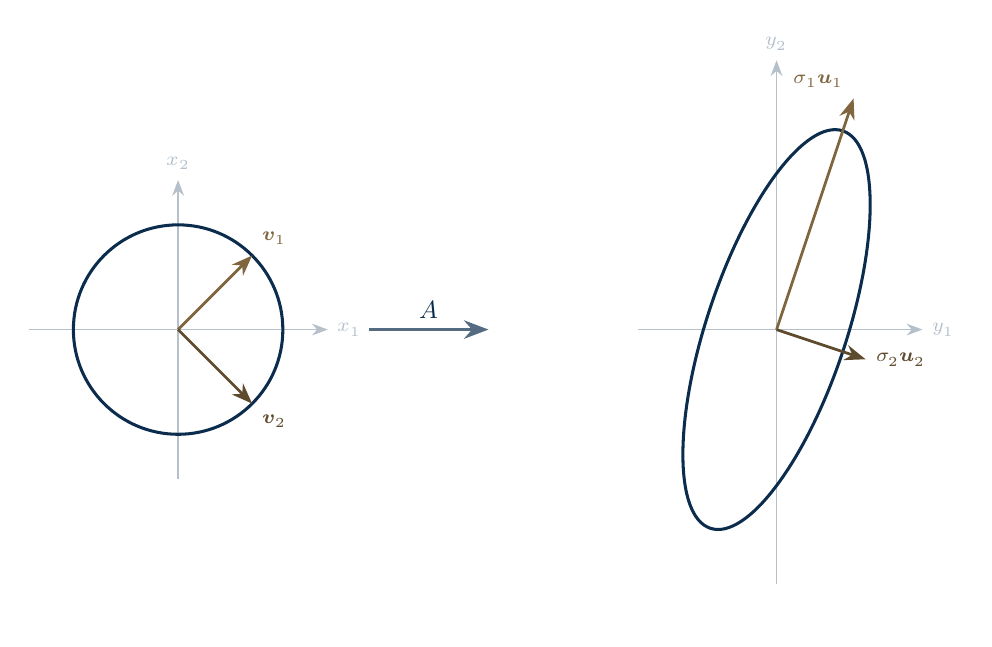
\begin{tikzpicture}[scale=0.95, >=Stealth]
  % ---- 左：定义域 ----
  \begin{scope}
    \draw[->, navy!30, line width=0.6pt] (-2.0,0)--(2.0,0) node[right,font=\scriptsize]{$x_1$};
    \draw[->, navy!30, line width=0.6pt] (0,-2.0)--(0,2.0) node[above,font=\scriptsize]{$x_2$};
    \draw[navy, line width=1.1pt] (0,0) circle (1.4);
    \draw[->, gold!75!black, line width=1pt] (0,0)--(0.99,0.99)
      node[above right,font=\scriptsize]{$\vv_1$};
    \draw[->, gold!55!black, line width=1pt] (0,0)--(0.99,-0.99)
      node[below right,font=\scriptsize]{$\vv_2$};
    \node[font=\small,text=navy] at (0,-2.45) {定义域：单位圆};
  \end{scope}
  % ---- 箭头 ----
  \draw[->, line width=1.3pt, navy!70] (2.55,0)--(4.15,0)
      node[midway,above,font=\small,text=navy]{$A$};
  % ---- 右：值域 ----
  \begin{scope}[shift={(8.0,0)}]
    \draw[->, navy!30, line width=0.6pt] (-1.85,0)--(1.95,0) node[right,font=\scriptsize]{$y_1$};
    \draw[->, navy!30, line width=0.6pt] (0,-3.4)--(0,3.6) node[above,font=\scriptsize]{$y_2$};
    \begin{scope}[rotate=71.565]
      \draw[navy, line width=1.1pt] (0,0) ellipse (2.8 and 0.933);
    \end{scope}
    \draw[->, gold!75!black, line width=1pt] (0,0)--(1.03,3.09)
      node[above left,font=\scriptsize]{$\sigma_1\bu_1$};
    \draw[->, gold!55!black, line width=1pt] (0,0)--(1.19,-0.397)
      node[right,font=\scriptsize]{$\sigma_2\bu_2$};
    \node[font=\small,text=navy] at (0.55,-3.75) {值域：椭圆};
  \end{scope}
\end{tikzpicture}
\caption{$2\times2$ 矩阵把单位圆映成椭圆。椭圆的两条半轴长度分别是两个奇异值
$\sigma_1=3\sqrt5\approx6.708$ 与 $\sigma_2=\sqrt5\approx2.236$，半轴方向分别是
$\bu_1$ 与 $\bu_2$。注意左右两图的比例尺不同：左图的圆半径与右图的短半轴在视觉上相近，
只是为了排版方便。}
\label{fig:circle-ellipse}
\end{figure}

图 \ref{fig:circle-ellipse} 揭示了一件重要的事：\textbf{任意可逆的 $2\times2$ 矩阵都
把单位圆变成椭圆}（退化情形下变成线段）。椭圆的形状完全由两个半轴的长度和方向决定，
而这两者正是我们要找的奇异值和奇异向量。

\subsection{为什么一定是椭圆}

这不是巧合。设 $\x$ 在单位圆上，$\y=A\x$。椭圆是“到两个定点距离之和为常数”的点集，
但更直接的说法是：椭圆是单位圆在仿射变换下的像。任何满秩方阵都是可逆线性变换，
它把圆映成椭圆；这个结论在 $n$ 维下同样成立——单位球面被映成\textbf{椭球面}。

椭球的主轴长度，衡量了矩阵在不同方向上“拉伸”了多少。最大的拉伸倍数就是
$\nrm{A}_2$，最小的拉伸倍数（$A$ 可逆时）就是 $1/\nrm{A^{-1}}_2$。二者的比值就是条件数。
一台机器如果某个方向几乎被压扁（$\sigma_r\approx0$），那么它在这个方向上就“几乎不可逆”，
这也是病态问题的几何来源。

\subsection{三步分解：旋转—拉伸—旋转}

既然 $A$ 把单位圆变成椭圆，我们就可以反过来，把 $A$ 的作用拆成三步：先转一下，
让椭圆的主轴对齐坐标轴；再沿坐标轴拉伸；最后转回去。这三步恰好对应
\begin{equation}
  A=U\Sigma V\T ,
\end{equation}
其中 $V\T$ 与 $U$ 是正交变换（旋转或反射），$\Sigma$ 是对角矩阵（沿坐标轴拉伸）。

\begin{figure}[htbp]
\centering
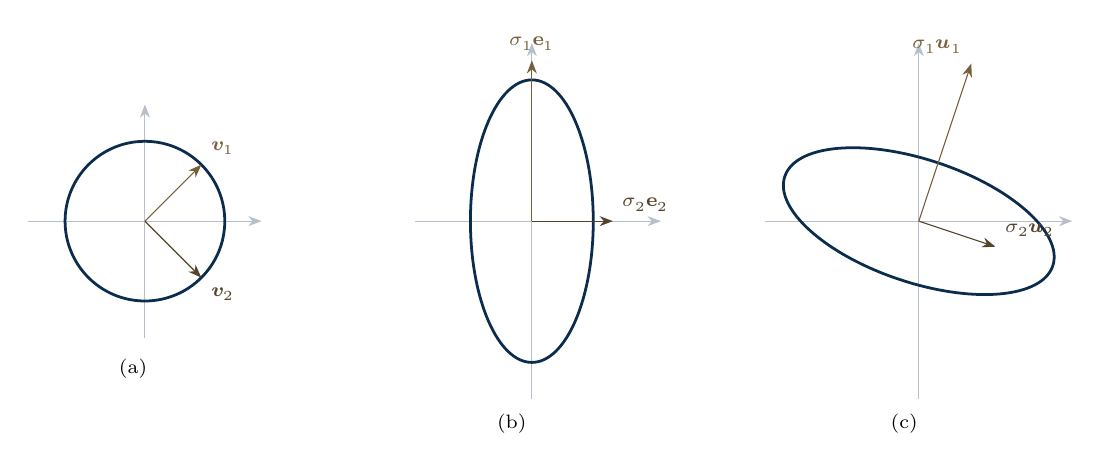
\begin{tikzpicture}[scale=0.78, >=Stealth]
  % (a) 单位圆
  \begin{scope}
    \draw[->, navy!30] (-1.9,0)--(1.9,0);
    \draw[->, navy!30] (0,-1.9)--(0,1.9);
    \draw[navy, line width=1pt] (0,0) circle (1.3);
    \draw[->, gold!70!black] (0,0)--(0.919,0.919) node[above right,font=\scriptsize]{$\vv_1$};
    \draw[->, gold!50!black] (0,0)--(0.919,-0.919) node[below right,font=\scriptsize]{$\vv_2$};
    \node[font=\scriptsize] at (0,-2.4) {(a) 单位圆};
  \end{scope}
  % (b) 轴对齐椭圆
  \begin{scope}[shift={(6.3,0)}]
    \draw[->, navy!30] (-1.9,0)--(2.1,0);
    \draw[->, navy!30] (0,-2.9)--(0,2.9);
    \draw[navy, line width=1pt] (0,0) ellipse (1 and 2.3);
    \draw[->, gold!70!black] (0,0)--(0,2.62) node[above,font=\scriptsize]{$\sigma_1\mathbf{e}_1$};
    \draw[->, gold!50!black] (0,0)--(1.32,0) node[above right,font=\scriptsize]{$\sigma_2\mathbf{e}_2$};
    \node[font=\scriptsize] at (0,-3.3) {(b) 沿坐标轴拉伸};
  \end{scope}
  % (c) 旋转后的椭圆
  \begin{scope}[shift={(12.6,0)}]
    \draw[->, navy!30] (-2.5,0)--(2.5,0);
    \draw[->, navy!30] (0,-2.9)--(0,2.9);
    \begin{scope}[rotate=71.565]
      \draw[navy, line width=1pt] (0,0) ellipse (1 and 2.3);
    \end{scope}
    \draw[->, gold!70!black] (0,0)--(0.855,2.566) node[above left,font=\scriptsize]{$\sigma_1\bu_1$};
    \draw[->, gold!50!black] (0,0)--(1.248,-0.416) node[above right,font=\scriptsize]{$\sigma_2\bu_2$};
    \node[font=\scriptsize] at (0,-3.3) {(c) 整体旋转};
  \end{scope}
\end{tikzpicture}
\caption{SVD 的三步分解。$V\T$ 先把 $(a)$ 中的正交方向 $\vv_1,\vv_2$ 转到坐标轴方向
$(b)$；$\Sigma$ 沿坐标轴分别拉伸 $\sigma_1$ 与 $\sigma_2$ 倍；$U$ 再把整个椭球旋到
$(c)$ 所示的最终朝向。图中为示意比例，未按 $A$ 的真实奇异值 $6.708:2.236$ 绘制。}
\label{fig:three-steps}
\end{figure}

\begin{insight}[一句话记住 SVD]
$A\x=(U\Sigma V\T)\x$ 的意思是：把 $\x$ 用 $\vv_1,\dots,\vv_n$ 这组正交坐标表示，
沿每个坐标轴拉伸 $\sigma_i$ 倍，再用 $\bu_1,\dots,\bu_m$ 这组正交坐标表示出来。
$V\T$ 负责“换到输入坐标系”，$U$ 负责“换到输出坐标系”，$\Sigma$ 负责“拉伸”。
\end{insight}

\subsection{退化情形：当椭圆被压扁}

如果 $\sigma_2=0$，椭圆退化成一条线段，$A$ 不可逆，$\rank(A)=1$。此时
$\vv_2$ 满足 $A\vv_2=\mathbf{0}$，即 $\vv_2$ 落在 $A$ 的零空间里。方向 $\vv_2$ 上的
一切信息都被压没了。

这不是病态，而是低秩矩阵的常态。图像、评分矩阵、文档—词频矩阵，它们的奇异值谱往往
是“少数几个很大，其余迅速趋近于零”。第 \ref{sec:lowrank} 节会说明，这正是低秩逼近
能够奏效的原因。

\subsection*{自检}
\begin{enumerate}
  \item 对式 \eqref{eq:example-A} 的 $A$，验证 $\nrm{A\x}_2$ 在
        $\vv_1=\frac{1}{\sqrt2}(1,1)\T$ 处取到最大值 $\sqrt{45}$。
        （提示：设 $\x=(\cos\theta,\sin\theta)\T$，把 $\nrm{A\x}_2^2$ 写成 $\theta$ 的函数。）
  \item 若 $A$ 是正交矩阵，$AS^1$ 是什么形状？它的奇异值是多少？
  \item 若 $A$ 把单位圆压成一条线段，$\det A$ 等于多少？
\end{enumerate}

% ============================================================
\section{奇异值分解的定义}\label{sec:def}
% ============================================================

几何直觉已经给出了 SVD 的轮廓，这一节把它写成严格的定义，并用一个
$3\times2$ 的例子把每一步都算出来。

\subsection{完整形式与约化形式}

\begin{defn}[奇异值分解]\label{def:svd}
设 $A\in\R^{m\times n}$，$\rank(A)=r\ge1$。若存在正交矩阵
$U\in\R^{m\times m}$、$V\in\R^{n\times n}$ 以及矩阵 $\Sigma\in\R^{m\times n}$，
使得
\begin{equation}\label{eq:svd-full}
  A=U\Sigma V\T ,
\end{equation}
其中 $\Sigma$ 只有对角元 $\sigma_1\ge\sigma_2\ge\cdots\ge\sigma_r>0$ 非零、其余元素全为零，
则称式 \eqref{eq:svd-full} 为 $A$ 的\textbf{奇异值分解}（SVD）。
\end{defn}

\begin{defn}[奇异值与奇异向量]\label{def:sv}
在上述分解中：
\begin{itemize}
  \item $\sigma_1,\dots,\sigma_r$ 称为 $A$ 的\textbf{奇异值}（singular values）；
  \item $U$ 的第 $i$ 列 $\bu_i$ 称为\textbf{左奇异向量}；
  \item $V$ 的第 $i$ 列 $\vv_i$ 称为\textbf{右奇异向量}。
\end{itemize}
约定奇异值按降序排列，且只统计非零的那些，因此“$r$ 个奇异值”指的就是 $r$ 个正奇异值。
\end{defn}

\begin{rem}[关于 $\Sigma$ 的形状]
当 $m\neq n$ 时，$\Sigma$ 不是方阵，而是与 $A$ 同型的长方形矩阵：
当 $m>n$ 时，它是上面 $n$ 行构成对角块、下面 $m-n$ 行全为零；
当 $m<n$ 时，它是左边 $m$ 列构成对角块、右边 $n-m$ 列全为零。
矩阵 $\Sigma$ 中零的个数远多于非零的个数——这正是 SVD 的“压缩”所在。
\end{rem}

在实际使用中，完整形式往往显得臃肿：$U$ 的后面 $m-r$ 列与 $V$ 的后面 $n-r$ 列
乘上零之后根本不起作用。于是有了下面两种更常用的写法。

\begin{defn}[约化 SVD 与截断 SVD]\label{def:thin}
沿用上面的记号，设 $U_r=[\bu_1,\dots,\bu_r]$，$V_r=[\vv_1,\dots,\vv_r]$，
$\Sigma_r=\diag(\sigma_1,\dots,\sigma_r)$，则
\begin{equation}\label{eq:svd-thin}
  A=U_r\Sigma_r V_r\T
\end{equation}
称为 $A$ 的\textbf{约化 SVD}（thin SVD 或 economy SVD）。
若只取前 $k<r$ 项，
\begin{equation}\label{eq:svd-trunc}
  A_k=U_k\Sigma_k V_k\T=\sum_{i=1}^{k}\sigma_i\bu_i\vv_i\T
\end{equation}
则称为 $A$ 的\textbf{截断 SVD}（truncated SVD），其中
$U_k=[\bu_1,\dots,\bu_k]$，$V_k=[\vv_1,\dots,\vv_k]$。
\end{defn}

\begin{table}[htbp]
\centering
\small
\caption{SVD 的三种写法}\label{tab:three-forms}
\renewcommand{\arraystretch}{1.4}
\begin{tabular}{@{}lccc@{}}
\toprule
 & \textbf{完整 SVD} & \textbf{约化 SVD} & \textbf{截断 SVD} \\
\midrule
表达式 & $A=U\Sigma V\T$ & $A=U_r\Sigma_r V_r\T$ & $A_k=U_k\Sigma_k V_k\T$ \\
$U$ 的尺寸 & $m\times m$ & $m\times r$ & $m\times k$ \\
$\Sigma$ 的尺寸 & $m\times n$ & $r\times r$ & $k\times k$ \\
$V$ 的尺寸 & $n\times n$ & $n\times r$ & $n\times k$ \\
是否精确 & 是 & 是 & 否（除非 $k\ge r$） \\
主要用途 & 理论推导 & 计算、压缩存储 & 降维、去噪、逼近 \\
\bottomrule
\end{tabular}
\end{table}

从表 \ref{tab:three-forms} 可以看出，约化 SVD 与完整 SVD 是同一个分解的不同“裁剪”，
而截断 SVD 是有损的：它主动丢掉了后面 $r-k$ 个分量。第 \ref{sec:lowrank} 节会说明，
这种丢弃在所有可能的丢弃方式中是\textbf{最优}的。

\subsection{手算一个 \texorpdfstring{$3\times2$}{3x2} 的例子}

为了让定义落地，我们把下面这个矩阵从里到外算一遍：
\begin{equation}\label{eq:example3x2}
  A=\begin{pmatrix}1&0\\0&1\\1&1\end{pmatrix}\in\R^{3\times2}.
\end{equation}

\paragraph{第一步：算 $A\T A$。}
\begin{equation}
  A\T A=
  \begin{pmatrix}1&0&1\\0&1&1\end{pmatrix}
  \begin{pmatrix}1&0\\0&1\\1&1\end{pmatrix}
  =\begin{pmatrix}2&1\\1&2\end{pmatrix}.
\end{equation}

\paragraph{第二步：求 $A\T A$ 的特征值。}
特征多项式为
$\det(A\T A-\lambda I)=(2-\lambda)^2-1=(\lambda-1)(\lambda-3)$，
故特征值为 $\lambda_1=3$，$\lambda_2=1$。两者都为正，说明 $\rank(A)=2$，$A$ 是列满秩的。

\paragraph{第三步：求单位特征向量。}
对 $\lambda_1=3$：解 $(A\T A-3I)\x=\mathbf{0}$，即
$\begin{pmatrix}-1&1\\1&-1\end{pmatrix}\x=\mathbf{0}$，得 $\x\propto(1,1)\T$，
单位化后 $\vv_1=\frac{1}{\sqrt2}(1,1)\T$。

对 $\lambda_2=1$：解 $\begin{pmatrix}1&1\\1&1\end{pmatrix}\x=\mathbf{0}$，
得 $\x\propto(1,-1)\T$，单位化后 $\vv_2=\frac{1}{\sqrt2}(1,-1)\T$。

两者内积为零，验证了谱定理的结论。

\paragraph{第四步：奇异值是特征值的平方根。}
\begin{equation}
  \sigma_1=\sqrt{\lambda_1}=\sqrt3\approx1.732,\qquad
  \sigma_2=\sqrt{\lambda_2}=1 .
\end{equation}

\paragraph{第五步：用 $\bu_i=A\vv_i/\sigma_i$ 算左奇异向量。}
\begin{align}
  A\vv_1&=\frac{1}{\sqrt2}\begin{pmatrix}1\\1\\2\end{pmatrix},
  &\bu_1&=\frac{A\vv_1}{\sigma_1}
  =\frac{1}{\sqrt2\cdot\sqrt3}\begin{pmatrix}1\\1\\2\end{pmatrix}
  =\frac{1}{\sqrt6}\begin{pmatrix}1\\1\\2\end{pmatrix},\\[4pt]
  A\vv_2&=\frac{1}{\sqrt2}\begin{pmatrix}1\\-1\\0\end{pmatrix},
  &\bu_2&=\frac{A\vv_2}{\sigma_2}
  =\frac{1}{\sqrt2}\begin{pmatrix}1\\-1\\0\end{pmatrix}.
\end{align}

\paragraph{第六步：补全 $U$ 的第三列。}
$\bu_1,\bu_2$ 已是 $\R^3$ 中的标准正交组，还差一个方向。取
\begin{equation}
  \bu_3=\frac{1}{\sqrt3}\begin{pmatrix}1\\1\\-1\end{pmatrix},
\end{equation}
直接验证 $\bu_3\T\bu_1=\bu_3\T\bu_2=0$ 且 $\nrm{\bu_3}=1$。
（也可以取反方向 $-\bu_3$，两种取法都合法，见 \ref{sec:unique} 节关于唯一性的讨论。）

\paragraph{第七步：写出三个矩阵并验证。}
\begin{equation}
  U=\begin{pmatrix}
  \frac{1}{\sqrt6}&\frac{1}{\sqrt2}&\frac{1}{\sqrt3}\\[3pt]
  \frac{1}{\sqrt6}&-\frac{1}{\sqrt2}&\frac{1}{\sqrt3}\\[3pt]
  \frac{2}{\sqrt6}&0&-\frac{1}{\sqrt3}
  \end{pmatrix},\quad
  \Sigma=\begin{pmatrix}\sqrt3&0\\0&1\\0&0\end{pmatrix},\quad
  V=\begin{pmatrix}
  \frac{1}{\sqrt2}&\frac{1}{\sqrt2}\\[3pt]
  \frac{1}{\sqrt2}&-\frac{1}{\sqrt2}
  \end{pmatrix}.
\end{equation}

验证 $(1,1)$ 元与 $(3,2)$ 元（其余元素同理）：
\begin{align}
  (U\Sigma V\T)_{11}
  &=\Big(\tfrac{1}{\sqrt2}\Big)\Big(\tfrac{1}{\sqrt2}\Big)
   +\Big(\tfrac{1}{\sqrt2}\Big)\Big(\tfrac{1}{\sqrt2}\Big)=1,\\
  (U\Sigma V\T)_{32}
  &=\Big(\tfrac{2}{\sqrt2}\Big)\Big(\tfrac{1}{\sqrt2}\Big)
   +0\cdot\Big(-\tfrac{1}{\sqrt2}\Big)=1 .
\end{align}
与 $A$ 的对应元素一致。$\Sigma$ 的第三行全为零，恰好对应 $\rank(A)=2<3$。

\begin{insight}[这个例子说明了什么]
$A$ 把 $\R^2$ 中的单位圆映成 $\R^3$ 中的椭圆，椭圆所在平面由 $\bu_1,\bu_2$ 张成，
半轴长度是 $\sqrt3$ 和 $1$。第三个方向 $\bu_3$ 垂直于这个平面，整个平面在 $\bu_3$
方向上的“厚度”为零——这就是 $\sigma_3=0$ 的几何含义。任何 $m\times n$ 矩阵的像都
落在 $\Span\{\bu_1,\dots,\bu_r\}$ 这个 $r$ 维子空间里。
\end{insight}

\subsection{外积形式：把矩阵拆成秩一矩阵之和}

把 $A=U\Sigma V\T$ 按列展开，可以得到最常用的一种写法：
\begin{equation}\label{eq:svd-outer}
  A=\sum_{i=1}^{r}\sigma_i\,\bu_i\vv_i\T .
\end{equation}

每一项 $\bu_i\vv_i\T$ 是一个 $m\times n$ 矩阵，它的每一列都是 $\bu_i$ 的倍数，
每一行都是 $\vv_i\T$ 的倍数，因此秩为 $1$。式 \eqref{eq:svd-outer} 说的是：
\textbf{任何矩阵都可以写成若干个秩一矩阵的加权和，权重就是奇异值。}

这个视角非常有用。它把矩阵的“信息量”分解成一个个独立的层：第一层
$\sigma_1\bu_1\vv_1\T$ 贡献最大，第二层次之，依此类推。奇异值下降得越快，说明少数几层
就能撑起整个矩阵，这就是“低秩”的量化含义。

% ============================================================
\section{存在性：为什么 SVD 一定存在}\label{sec:exist}
% ============================================================

定义只是说“如果存在这样的分解，就叫它 SVD”，还没有回答它是否真的存在。
这一节给出构造性证明：不仅证明存在，还顺便给出了计算方法。

\subsection{证明路线图}

证明分三步，每一步只用一个工具：

\begin{enumerate}
  \item \textbf{对 $A\T A$ 用谱定理。} 由命题 \ref{prop:ata-psd}，$A\T A$ 对称半正定，
        于是有 $n$ 个非负实特征值和一组标准正交特征向量 $\vv_1,\dots,\vv_n$。
  \item \textbf{构造 $\bu_i$。} 对前 $r$ 个正特征值，令
        $\bu_i=A\vv_i/\sigma_i$，并证明它们恰好是单位正交的。
  \item \textbf{补全并验证。} 把 $\{\bu_1,\dots,\bu_r\}$ 扩充成 $\R^m$ 的标准正交基，
        然后验证 $A=U\Sigma V\T$ 在基向量上成立。
\end{enumerate}

这个证明的美妙之处在于：它不需要任何高深工具，只需要“对称矩阵可正交对角化”这一条，
剩下的都是计算。

\subsection{第一步：\texorpdfstring{$A\T A$}{AᵀA} 的特征分解}

\begin{lemma}\label{lem:eig}
设 $A\in\R^{m\times n}$，$\rank(A)=r$。则 $A\T A$ 的特征值可以排成
\begin{equation}
  \lambda_1\ge\lambda_2\ge\cdots\ge\lambda_r>0=\lambda_{r+1}=\cdots=\lambda_n ,
\end{equation}
对应的单位特征向量 $\vv_1,\dots,\vv_n$ 构成 $\R^n$ 的标准正交基，且
$A\T A\vv_i=\lambda_i\vv_i$。此外，$\vv_{r+1},\dots,\vv_n$ 张成 $\Null(A)$。
\end{lemma}

\begin{proof}
由命题 \ref{prop:ata-psd}，$A\T A$ 对称半正定，特征值全为非负实数。由谱定理，
存在标准正交特征向量组 $\vv_1,\dots,\vv_n$。按特征值降序排列，正特征值的个数记为 $r'$。

对任意 $i$，$\lambda_i=0$ 等价于 $A\T A\vv_i=\mathbf{0}$，由命题 \ref{prop:ata-psd}
的式 \eqref{eq:ata-null} 等价于 $A\vv_i=\mathbf{0}$。因此零特征值对应的特征向量恰好
张成 $\Null(A)$，其个数为 $n-\rank(A)=n-r$。所以 $r'=r$。
\end{proof}

\begin{rem}
这个引理同时说明了两件事：奇异值的平方就是 $A\T A$ 的特征值；右奇异向量就是
$A\T A$ 的特征向量。这两条是后面所有计算的基础。
\end{rem}

\subsection{第二步：构造左奇异向量}

\begin{lemma}\label{lem:u-orth}
对 $i=1,\dots,r$，定义
\begin{equation}
  \bu_i=\frac{A\vv_i}{\sigma_i},\qquad \sigma_i=\sqrt{\lambda_i}>0 .
\end{equation}
则 $\bu_1,\dots,\bu_r$ 是 $\R^m$ 中的标准正交组。
\end{lemma}

\begin{proof}
\textbf{长度：}由 $\vv_i$ 是 $A\T A$ 的单位特征向量，
\begin{equation}
  \nrm{A\vv_i}_2^2=(A\vv_i)\T(A\vv_i)=\vv_i\T A\T A\vv_i=\lambda_i\nrm{\vv_i}_2^2=\sigma_i^2 ,
\end{equation}
故 $\nrm{\bu_i}_2=\nrm{A\vv_i}_2/\sigma_i=1$。

\textbf{正交：}对 $i\neq j$，
\begin{equation}
  \bu_i\T\bu_j=\frac{(A\vv_i)\T(A\vv_j)}{\sigma_i\sigma_j}
  =\frac{\vv_i\T A\T A\vv_j}{\sigma_i\sigma_j}
  =\frac{\lambda_j\,\vv_i\T\vv_j}{\sigma_i\sigma_j}=0,
\end{equation}
最后一步用了 $\vv_i\T\vv_j=0$。
\end{proof}

\begin{rem}
这里用到了一个容易被忽略的事实：$A\vv_i$ 与 $A\vv_j$ 的正交性，是由 $\vv_i$ 与 $\vv_j$
关于 $A\T A$ 的正交性“传递”过来的。这种“把正交性从一个空间搬到另一个空间”的技巧，
在矩阵分析里非常常见。
\end{rem}

\subsection{第三步：补全并验证}

\begin{thm}[奇异值分解的存在性]\label{thm:svd-exist}
设 $A\in\R^{m\times n}$，$\rank(A)=r\ge1$。则存在正交矩阵
$U\in\R^{m\times m}$、$V\in\R^{n\times n}$ 与 $m\times n$ 的对角矩阵 $\Sigma$，
使得 $A=U\Sigma V\T$。
\end{thm}

\begin{proof}
取 $V=[\vv_1,\dots,\vv_n]$，其中 $\vv_i$ 是引理 \ref{lem:eig} 给出的标准正交特征向量，
此时 $V$ 是正交矩阵。

取 $\bu_1,\dots,\bu_r$ 如引理 \ref{lem:u-orth}，它们构成 $\R^m$ 中的标准正交组。
由 Gram--Schmidt 过程，可以把它扩充为 $\R^m$ 的标准正交基
$\bu_1,\dots,\bu_r,\bu_{r+1},\dots,\bu_m$，令 $U=[\bu_1,\dots,\bu_m]$，
则 $U$ 也是正交矩阵。

令 $\Sigma\in\R^{m\times n}$ 的对角元为 $\sigma_1,\dots,\sigma_r$，其余为零。
下面验证 $A=U\Sigma V\T$。由于 $\{\vv_1,\dots,\vv_n\}$ 是 $\R^n$ 的一组基，
只需验证两边作用在每个 $\vv_j$ 上结果相同。

\textbf{情形一：$j\le r$。}此时 $\sigma_j>0$，有
\begin{equation}
  U\Sigma V\T\vv_j=U\Sigma\mathbf{e}_j=U(\sigma_j\mathbf{e}_j)=\sigma_j\bu_j=A\vv_j ,
\end{equation}
最后一步正是 $\bu_j$ 的定义。

\textbf{情形二：$j>r$。}此时 $\lambda_j=0$，由引理 \ref{lem:eig}，$\vv_j\in\Null(A)$，
故 $A\vv_j=\mathbf{0}$；而 $\Sigma\mathbf{e}_j=\mathbf{0}$，故
$U\Sigma V\T\vv_j=\mathbf{0}$。两边也相同。

两个线性映射在基上处处相同，故恒等，即 $A=U\Sigma V\T$。
\end{proof}

\begin{keybox}[证明的结构]
整个证明可以浓缩成一句话：\textbf{把 $A\T A$ 的特征分解当作“原料”，
用 $A\vv_i/\sigma_i$ 造出另一半，再用基向量检验}。
这个构造过程也提示了算法：只要能算 $A\T A$ 的特征分解，就能算 SVD。
当然，实际计算不会真这么做（原因见第 \ref{sec:compute} 节），但思路是对的。
\end{keybox}

\subsection{秩、零空间与奇异值}

\begin{thm}\label{thm:rank-sv}
设 $A=U\Sigma V\T$ 是 $A\in\R^{m\times n}$ 的 SVD，则
\begin{equation}
  \rank(A)=\#\{i:\sigma_i>0\}=r .
\end{equation}
\end{thm}

\begin{proof}
$U$ 与 $V$ 都是正交矩阵，因而可逆，左乘或右乘可逆矩阵不改变秩，故
$\rank(A)=\rank(\Sigma)$。而 $\Sigma$ 只有前 $r$ 个对角元非零，其余元素全为零，
其秩显然为 $r$。
\end{proof}

\begin{cor}\label{cor:null}
在同样的记号下，
\begin{align}
  \Null(A)&=\Span\{\vv_{r+1},\dots,\vv_n\}, & \dim\Null(A)&=n-r,\\
  \Col(A)&=\Span\{\bu_1,\dots,\bu_r\}, & \dim\Col(A)&=r .
\end{align}
\end{cor}

\begin{proof}
第一式已由引理 \ref{lem:eig} 得到。第二式：任意 $\x$ 可写成
$\x=\sum_{j=1}^{n}c_j\vv_j$，则
$A\x=\sum_{j=1}^{r}c_j\sigma_j\bu_j$，落在他 $\Span\{\bu_1,\dots,\bu_r\}$ 中；
反过来取 $\x=\vv_i/\sigma_i$（$i\le r$）即得 $\bu_i$，故两者相等。
\end{proof}

\begin{rem}
推论 \ref{cor:null} 给出了一个非常实用的结论：\textbf{矩阵的秩等于非零奇异值的个数}。
在数值计算中，由于浮点误差，理论上为零的奇异值往往算出来是 $10^{-16}$ 量级的小数，
因此常把小于某个阈值（如 $\sigma_1\cdot\max(m,n)\cdot\varepsilon_{\text{mach}}$）的
奇异值视为零。这就是“数值秩”的概念，第 \ref{sec:compute} 节还会讨论。
\end{rem}

\subsection{唯一性：哪些东西是确定的}\label{sec:unique}

\begin{thm}[SVD 的唯一性]\label{thm:unique}
奇异值 $\sigma_1,\dots,\sigma_r$ 由 $A$ 唯一确定。若 $\sigma_1>\cdots>\sigma_r>0$
且互不相同，则 $\vv_i$ 与 $\bu_i$（$i\le r$）在相差一个符号的意义下唯一；
若存在重奇异值，则对应的奇异向量子空间唯一，但子空间内的正交基可以任意旋转。
零奇异值对应的 $\vv_j$（$j>r$）与 $\bu_j$（$j>r$）完全不确定。
\end{thm}

\begin{proof}[证明要点]
奇异值是 $A\T A$ 的特征值的平方根，而特征值由 $A\T A$ 唯一确定，故奇异值唯一。
若 $\lambda_i$ 是单重特征值，其特征子空间是一维的，单位向量只有 $\pm\vv_i$ 两种取法。
若 $\lambda_i$ 是 $q$ 重特征值，对应特征子空间是 $q$ 维的，其中任意一组标准正交基都
可以作为 $\vv$ 的相应列，此时 $\bu$ 也随之确定（因为 $\bu=A\vv/\sigma$）。
零特征值对应的子空间是 $\Null(A)$，与 $\Col(A)$ 的正交补无任何约束关系，故完全任意。
\end{proof}

\begin{warnbox}[符号不确定性会带来麻烦]
同一个矩阵，NumPy 与 MATLAB 算出的 $\bu_i$、$\vv_i$ 可能差一个负号，甚至同一份代码
在不同 BLAS 后端上也可能不同。如果你在比较两组奇异向量（比如做实验复现），
不要直接比较向量本身，而应比较 $\abs{\bu_i\T\hat{\bu}_i}$，或者比较投影矩阵
$\bu_i\bu_i\T$。另外，若 $\sigma_i$ 有重根，连“第 $i$ 个奇异向量”这个说法本身
都没有意义——有意义的是那个不变子空间。
\end{warnbox}

% ============================================================
\section{基本性质：范数、秩与条件数}\label{sec:prop}
% ============================================================

这一节把 SVD 与线性代数里几个最重要的量联系起来。结论本身都很简洁，
但每一个在后面都会反复出现。

\subsection{奇异值与特征值的关系}

\begin{prop}\label{prop:sv-eig}
设 $A\in\R^{m\times n}$，奇异值为 $\sigma_1\ge\cdots\ge\sigma_r>0$，则
\begin{enumerate}
  \item $\sigma_i^2$ 是 $A\T A$（也是 $AA\T$）的非零特征值；
  \item 若 $A$ 是 $n$ 阶方阵，其特征值为 $\lambda_1,\dots,\lambda_n$（可能是复数），则
        $\abs{\lambda_i}\le\sigma_1$，且 $\prod_i\abs{\lambda_i}\le\prod_i\sigma_i$；
  \item 若 $A$ 是对称矩阵，则 $\sigma_i=\abs{\lambda_i}$，其中 $\lambda_i$ 按绝对值降序排列；
  \item 若 $A$ 是正交矩阵，则所有奇异值都等于 $1$。
\end{enumerate}
\end{prop}

\begin{proof}
(1) 由 $A\T A=V\Sigma\T\Sigma V\T$ 即得：$A\T A$ 与 $\Sigma\T\Sigma$ 相似
（更准确地说，是正交相似），故特征值相同，而 $\Sigma\T\Sigma$ 的对角元正是 $\sigma_i^2$。

(3) 若 $A$ 对称，由谱定理 $A=Q\Lambda Q\T$，取 $U=Q$、$V=Q\,\mathrm{sgn}(\Lambda)$
（把负特征值对应的列反号），即得 $A=U\abs{\Lambda}V\T$，故 $\sigma_i=\abs{\lambda_i}$。

(4) 若 $A$ 正交，则 $A\T A=I$，特征值全为 $1$，故 $\sigma_i=1$。

(2) 的证明需要用到特征值的变分刻画，这里从略；直观上，$\sigma_1$ 是矩阵在
\textbf{任何}方向上的最大拉伸倍数，而 $\lambda_1$ 只是某个特定方向上的拉伸倍数，
自然有 $\abs{\lambda_1}\le\sigma_1$。
\end{proof}

\begin{warnbox}[奇异值不是特征值的绝对值]
对一般的方阵，“$\sigma_i=\abs{\lambda_i}$”是\textbf{错的}。例如
$A=\bigl(\begin{smallmatrix}0&1\\0&0\end{smallmatrix}\bigr)$ 的特征值全为 $0$，但奇异值是 $1$ 和 $0$。
只有当 $A$ 对称（或更一般地，正规）时，两者才有上述关系。
正确的普遍关系是 $\sigma_i^2=\lambda_i(A\T A)$，而不是 $\lambda_i(A)^2$。
\end{warnbox}

\subsection{三种矩阵范数}

\begin{defn}[矩阵范数]\label{def:norms}
对 $A\in\R^{m\times n}$，定义
\begin{align}
  \nrm{A}_2&=\max_{\nrm{\x}_2=1}\nrm{A\x}_2
  &&\text{（谱范数，spectral norm）},\\
  \nrm{A}_F&=\Big(\sum_{i=1}^{m}\sum_{j=1}^{n}A_{ij}^2\Big)^{1/2}
  &&\text{（Frobenius 范数）},\\
  \nrm{A}_*&=\sum_{i=1}^{r}\sigma_i
  &&\text{（核范数，nuclear norm）}.
\end{align}
\end{defn}

\begin{thm}\label{thm:norms}
设 $A=U\Sigma V\T$，则
\begin{equation}
  \nrm{A}_2=\sigma_1,\qquad
  \nrm{A}_F=\Big(\sum_{i=1}^{r}\sigma_i^2\Big)^{1/2},\qquad
  \nrm{A}_*=\sum_{i=1}^{r}\sigma_i .
\end{equation}
\end{thm}

\begin{proof}
\textbf{谱范数。}对任意 $\x$，令 $\y=V\T\x$。由于 $V$ 正交，$\nrm{\y}_2=\nrm{\x}_2$，且
\begin{equation}
  \nrm{A\x}_2=\nrm{U\Sigma V\T\x}_2=\nrm{\Sigma\y}_2
  =\Big(\sum_{i=1}^{r}\sigma_i^2y_i^2\Big)^{1/2}
  \le\sigma_1\Big(\sum_{i=1}^{n}y_i^2\Big)^{1/2}=\sigma_1\nrm{\x}_2 .
\end{equation}
取 $\x=\vv_1$，则 $\y=\mathbf{e}_1$，$\nrm{A\vv_1}_2=\sigma_1$，故上界可取到。

\textbf{Frobenius 范数。}利用 $\nrm{A}_F^2=\tr(A\T A)$ 与迹的轮换不变性：
\begin{equation}
  \nrm{A}_F^2=\tr(V\Sigma\T U\T U\Sigma V\T)=\tr(V\Sigma\T\Sigma V\T)
  =\tr(\Sigma\T\Sigma V\T V)=\tr(\Sigma\T\Sigma)=\sum_{i=1}^{r}\sigma_i^2 .
\end{equation}

\textbf{核范数。}由定义 $\nrm{A}_*=\tr\big((A\T A)^{1/2}\big)$，而
$(A\T A)^{1/2}=V\Sigma V\T$（在秩 $r$ 的子空间上），故迹为 $\sum_i\sigma_i$。
\end{proof}

\begin{insight}[三个范数在说什么]
$\nrm{A}_2$ 只看\textbf{最大的那一个}奇异值，是“最坏情况”的放大倍数；
$\nrm{A}_F$ 把所有奇异值\textbf{平方求和}，更像“平均能量”；
$\nrm{A}_*$ 把所有奇异值\textbf{直接相加}，对大奇异值不如平方敏感，
因此常被用作“低秩”的凸松弛——它比秩函数好优化得多。
\end{insight}

\begin{rem}
$\nrm{A}_F$ 与 $\nrm{A}_2$ 满足
$\nrm{A}_2\le\nrm{A}_F\le\sqrt{r}\,\nrm{A}_2$，
因为 $\sigma_1^2\le\sum_i\sigma_i^2\le r\sigma_1^2$。
这两个不等式在估计误差时经常用到。
\end{rem}

\subsection{四个基本子空间}

线性代数有“四个基本子空间”之说：列空间、零空间、行空间、左零空间。SVD 把它们的
一组标准正交基直接送到你手上。

\begin{thm}[四个基本子空间的正交基]\label{thm:four-subspaces}
设 $A=U\Sigma V\T$，$\rank(A)=r$，则
\begin{align}
  \Row(A)&=\Span\{\vv_1,\dots,\vv_r\}, & \dim\Row(A)&=r,\\
  \Null(A)&=\Span\{\vv_{r+1},\dots,\vv_n\}, & \dim\Null(A)&=n-r,\\
  \Col(A)&=\Span\{\bu_1,\dots,\bu_r\}, & \dim\Col(A)&=r,\\
  \Null(A\T)&=\Span\{\bu_{r+1},\dots,\bu_m\}, & \dim\Null(A\T)&=m-r .
\end{align}
并且 $\Row(A)\perp\Null(A)$，$\Col(A)\perp\Null(A\T)$，
$\R^n=\Row(A)\oplus\Null(A)$，$\R^m=\Col(A)\oplus\Null(A\T)$。
\end{thm}

\begin{proof}
前两式即推论 \ref{cor:null}。第三式：$\Col(A)=\{A\x\}=\{\sum_{i\le r}\sigma_ic_i\bu_i\}$，
其中 $c_i=\vv_i\T\x$ 可取任意值，故等于 $\Span\{\bu_1,\dots,\bu_r\}$。
第四式对 $A\T=V\Sigma\T U\T$ 用第三式的结论即可。
正交性来自 $\vv_i$ 之间、$\bu_i$ 之间的正交关系。
\end{proof}

\begin{figure}[htbp]
\centering
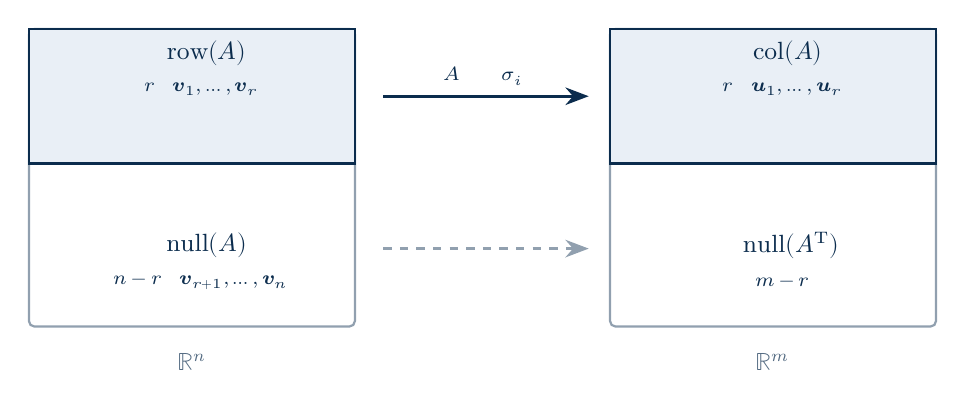
\begin{tikzpicture}[scale=0.9, >=Stealth]
  % 左空间 R^n
  \draw[navy!45, line width=0.8pt, rounded corners=2pt] (0,0) rectangle (4.6,4.2);
  \draw[navy, line width=0.9pt, fill=navypale] (0,2.3) rectangle (4.6,4.2);
  \node[font=\small, text=navy] at (2.3,3.85) {行空间 $\Row(A)$};
  \node[font=\scriptsize, text=navy] at (2.3,3.35) {维数 $r$，基 $\vv_1,\dots,\vv_r$};
  \node[font=\small, text=navy] at (2.3,1.15) {零空间 $\Null(A)$};
  \node[font=\scriptsize, text=navy] at (2.3,0.62) {维数 $n-r$，基 $\vv_{r+1},\dots,\vv_n$};
  \node[font=\small, text=navy!70] at (2.3,-0.5) {$\R^{n}$};
  % 右空间 R^m
  \begin{scope}[shift={(8.2,0)}]
  \draw[navy!45, line width=0.8pt, rounded corners=2pt] (0,0) rectangle (4.6,4.2);
  \draw[navy, line width=0.9pt, fill=navypale] (0,2.3) rectangle (4.6,4.2);
  \node[font=\small, text=navy] at (2.3,3.85) {列空间 $\Col(A)$};
  \node[font=\scriptsize, text=navy] at (2.3,3.35) {维数 $r$，基 $\bu_1,\dots,\bu_r$};
  \node[font=\small, text=navy] at (2.3,1.15) {左零空间 $\Null(A\T)$};
  \node[font=\scriptsize, text=navy] at (2.3,0.62) {维数 $m-r$};
  \node[font=\small, text=navy!70] at (2.3,-0.5) {$\R^{m}$};
  \end{scope}
  % 中间映射
  \draw[->, line width=1.2pt, navy] (5.0,3.25)--(7.9,3.25)
      node[midway, above, font=\scriptsize, text=navy] {$A$ 同构（缩放 $\sigma_i$）};
  \draw[->, line width=1.2pt, navy!45, dashed] (5.0,1.1)--(7.9,1.1)
      node[midway, above, font=\scriptsize, text=navy!60] {映为零};
\end{tikzpicture}
\caption{SVD 与四个基本子空间。$A$ 把行空间一一映到列空间（在基的意义下只差缩放
$\sigma_i$），把零空间整个压成原点。两个空间的维数之和分别为 $n$ 与 $m$。}
\label{fig:subspaces}
\end{figure}

图 \ref{fig:subspaces} 值得多看一会儿。它解释了为什么 SVD 被称为“矩阵的解剖图”：
$A$ 这个映射的全部行为，被 $r$ 个缩放因子和两组正交基完全描述干净了。

\subsection{条件数与病态问题}

\begin{defn}[条件数]\label{def:cond}
对可逆方阵 $A$，定义条件数
\begin{equation}
  \kappa(A)=\nrm{A}_2\nrm{A^{-1}}_2=\frac{\sigma_1}{\sigma_r}.
\end{equation}
对一般矩阵，用伪逆代替逆，$\kappa(A)=\sigma_1/\sigma_r$（$r=\rank(A)$）。
\end{defn}

\begin{prop}\label{prop:cond-square}
对任意 $A$，$\kappa(A\T A)=\kappa(A)^2$。
\end{prop}

\begin{proof}
$A\T A$ 的奇异值是 $A$ 的奇异值的平方，故
$\kappa(A\T A)=\sigma_1^2/\sigma_r^2=\kappa(A)^2$。
\end{proof}

条件数衡量的是“椭圆有多扁”。$\kappa=1$ 时椭圆的半轴一样长（所有方向拉伸相同，
$A$ 是正交矩阵的倍数）；$\kappa$ 很大时椭圆被压成很细的一条，某些方向的输入几乎
无法从输出中恢复。

\begin{keybox}[条件数的实际含义]
若 $\kappa(A)=10^{k}$，则在双精度（约 $16$ 位十进制有效数字）下，求解 $A\x=\bb$
大约会损失 $k$ 位有效数字。$\kappa=10^{12}$ 时，结果里只剩 4 位可信。
这不是算法不够好，而是问题本身对扰动敏感——任何用有限精度计算的方法都躲不开。
\end{keybox}

\subsection{行列式与迹}

\begin{prop}\label{prop:det}
设 $A$ 为 $n$ 阶方阵，则
\begin{equation}
  \abs{\det(A)}=\prod_{i=1}^{n}\sigma_i,\qquad
  \nrm{A}_F^2=\tr(A\T A)=\sum_{i=1}^{n}\sigma_i^2 .
\end{equation}
\end{prop}

\begin{proof}
$\det(A)=\det(U)\det(\Sigma)\det(V\T)$，而 $\det(U),\det(V)=\pm1$，
$\det(\Sigma)=\prod_i\sigma_i$（零奇异值使行列式为零，两边一致）。
第二式即定理 \ref{thm:norms} 的 Frobenius 部分。
\end{proof}

\begin{rem}
$\abs{\det A}$ 的几何意义是“体积放大倍数”：单位立方体经 $A$ 作用后变成平行六面体，
体积为 $\prod_i\sigma_i$。这个平行六面体在最长的方向被拉伸 $\sigma_1$ 倍，
在最扁的方向被压缩 $\sigma_n$ 倍——条件数正是这两个倍数的比。
\end{rem}

\subsection*{自检}
\begin{enumerate}
  \item 若 $A$ 的所有奇异值相等且非零，$A$ 一定是什么形式的矩阵？
  \item 证明 $\nrm{A}_2\le\nrm{A}_F\le\sqrt{r}\nrm{A}_2$。
  \item 一个 $3\times3$ 矩阵的奇异值为 $100,10,0.1$，它的条件数是多少？
        若用双精度求解 $A\x=\bb$，大约还剩几位有效数字？
\end{enumerate}

% ============================================================
\section{低秩逼近：Eckart--Young 定理}\label{sec:lowrank}
% ============================================================

前面反复提到“截断 SVD 是最优的低秩逼近”，这一节把它证明出来。
这是 SVD 在工程上最重要的性质，没有之一。

\subsection{为什么追求低秩}

一个 $m\times n$ 矩阵需要 $mn$ 个数才能存下。若它的秩为 $k$，用截断 SVD 存储
只需要 $k(m+n+1)$ 个数：$k$ 个奇异值，$U_k$ 的 $mk$ 个元素，$V_k$ 的 $nk$ 个元素。
当 $k\ll\min(m,n)$ 时，这是数量级的节省。

低秩还有别的意义：

\begin{itemize}
  \item \textbf{去噪}：真实信号往往是低秩的，噪声是满秩的。截断掉小奇异值，就滤掉了噪声。
  \item \textbf{泛化}：在推荐系统里，“用户—物品”矩阵若近似低秩，意味着用户的偏好可以由
        少数几个潜在因子解释，从而能预测缺失的评分。
  \item \textbf{压缩}：图像、音频、神经网络的权重，都可以用低秩矩阵近似存储。
\end{itemize}

问题在于：给定 $k$，怎样找一个秩不超过 $k$ 的矩阵 $B$，使 $\nrm{A-B}$ 最小？
Eckart--Young 定理的回答是：\textbf{直接截断 SVD，不用再找}。

\subsection{定理的陈述}

\begin{thm}[Eckart--Young，1936]\label{thm:eckart-young}
设 $A\in\R^{m\times n}$ 的 SVD 为 $A=\sum_{i=1}^{r}\sigma_i\bu_i\vv_i\T$，
对 $1\le k<r$ 定义截断 SVD
\begin{equation}
  A_k=\sum_{i=1}^{k}\sigma_i\bu_i\vv_i\T .
\end{equation}
则对任意满足 $\rank(B)\le k$ 的 $B\in\R^{m\times n}$，有
\begin{align}
  \nrm{A-B}_2&\ge\sigma_{k+1}, \label{eq:ey-spectral}\\
  \nrm{A-B}_F&\ge\Big(\sum_{i=k+1}^{r}\sigma_i^2\Big)^{1/2}, \label{eq:ey-fro}
\end{align}
且 $B=A_k$ 同时使两式取等号。换言之，$A_k$ 既是谱范数意义下、也是 Frobenius 范数
意义下的\textbf{最佳秩 $k$ 逼近}。
\end{thm}

定理里有两个独立的结论，分别对应两种“误差”的定义。谱范数关心最坏方向上的误差，
F 范数关心总体平方误差。两者给出的最优解恰好是同一个 $A_k$，这一点并不平凡。

\subsection{谱范数情形的证明}

这个证明只需要一个巧妙的维数论证。

\begin{proof}[式 \eqref{eq:ey-spectral} 的证明]
设 $B$ 满足 $\rank(B)\le k$。由于 $B$ 是 $m\times n$ 矩阵，其零空间维数至少为 $n-k$：
\begin{equation}
  \dim\Null(B)=n-\rank(B)\ge n-k .
\end{equation}
另一方面，考虑由前 $k+1$ 个右奇异向量张成的子空间
$W=\Span\{\vv_1,\dots,\vv_{k+1}\}$，其维数为 $k+1$（因为对应的奇异值都为正，
这些向量线性无关）。

两个子空间都住在 $\R^n$ 里，维数之和为
$(n-k)+(k+1)=n+1>n$，故必有非零交叠：
\begin{equation}
  \dim\big(\Null(B)\cap W\big)\ge 1 .
\end{equation}

取交集中一个单位向量 $\mathbf{w}$。它有两个身份：

\textbf{身份一：}$\mathbf{w}\in\Null(B)$，故 $B\mathbf{w}=\mathbf{0}$，于是
$(A-B)\mathbf{w}=A\mathbf{w}$。

\textbf{身份二：}$\mathbf{w}\in W$，故可写成
$\mathbf{w}=\sum_{i=1}^{k+1}c_i\vv_i$，且 $\sum_{i=1}^{k+1}c_i^2=\nrm{\mathbf{w}}^2=1$。

把 $A\mathbf{w}$ 用 SVD 展开：
\begin{equation}
  A\mathbf{w}=\sum_{i=1}^{k+1}c_iA\vv_i=\sum_{i=1}^{k+1}c_i\sigma_i\bu_i .
\end{equation}
由于 $\bu_i$ 两两正交，
\begin{equation}
  \nrm{A\mathbf{w}}_2^2=\sum_{i=1}^{k+1}c_i^2\sigma_i^2
  \ge\sigma_{k+1}^2\sum_{i=1}^{k+1}c_i^2=\sigma_{k+1}^2 .
\end{equation}
（这里用了 $\sigma_i\ge\sigma_{k+1}$ 对 $i\le k+1$ 成立。）

于是
\begin{equation}
  \nrm{A-B}_2=\max_{\nrm{\x}=1}\nrm{(A-B)\x}_2
  \ge\nrm{(A-B)\mathbf{w}}_2=\nrm{A\mathbf{w}}_2\ge\sigma_{k+1} .
\end{equation}

最后验证等号：$A-A_k=\sum_{i=k+1}^{r}\sigma_i\bu_i\vv_i\T$，它的最大奇异值正是
$\sigma_{k+1}$，故 $\nrm{A-A_k}_2=\sigma_{k+1}$。
\end{proof}

\begin{insight}[证明的核心思想]
任意一个秩不超过 $k$ 的矩阵，都必然“看不见”某个 $k+1$ 维的方向组合——
它的零空间太大了，躲不开前 $k+1$ 个奇异方向张成的子空间。
在那个躲不开的方向上，$B$ 什么也做不了，只能让 $A$ 自己去拉伸，
于是误差至少是 $\sigma_{k+1}$。
\end{insight}

\subsection{Frobenius 范数情形的证明}

F 范数的情形需要一个关于迹的不等式。

\begin{lemma}[von Neumann 迹不等式]\label{lem:von-neumann}
对任意 $A,B\in\R^{m\times n}$，
\begin{equation}
  \abs{\tr(A\T B)}\le\sum_{i=1}^{\min(m,n)}\sigma_i(A)\sigma_i(B).
\end{equation}
\end{lemma}

\begin{proof}[证明思路]
令 $A=U\Sigma V\T$，$B=P\Lambda Q\T$ 为各自的 SVD，则
\begin{equation}
  \tr(A\T B)=\tr(V\Sigma U\T P\Lambda Q\T)=\tr\big(\Sigma\,(U\T P)\,\Lambda\,(Q\T V)\big).
\end{equation}
记 $X=U\T P$、$Y=Q\T V$，两者都是正交矩阵。于是问题化为：对正交的 $X,Y$ 与非负对角阵
$\Sigma,\Lambda$，证明 $\abs{\tr(\Sigma X\Lambda Y)}\le\sum_i\sigma_i\lambda_i$。
这可以用重排不等式（Hardy--Littlewood--Pólya）证明，此处从略。
\end{proof}

\begin{proof}[式 \eqref{eq:ey-fro} 的证明]
设 $\rank(B)\le k$，记 $a_i=\sigma_i(A)$，$b_i=\sigma_i(B)$。由于 $\rank(B)\le k$，
当 $i>k$ 时 $b_i=0$。展开平方：
\begin{align}
  \nrm{A-B}_F^2
  &=\nrm{A}_F^2-2\tr(A\T B)+\nrm{B}_F^2 \notag\\
  &\ge\sum_{i=1}^{r}a_i^2-2\sum_{i=1}^{k}a_ib_i+\sum_{i=1}^{k}b_i^2
  \qquad\text{（引理 \ref{lem:von-neumann}）}\notag\\
  &=\sum_{i=k+1}^{r}a_i^2+\sum_{i=1}^{k}(a_i-b_i)^2
  \notag\\
  &\ge\sum_{i=k+1}^{r}a_i^2 . \label{eq:fro-bound}
\end{align}
最后一步因为平方项非负。对 $B=A_k$，有 $b_i=a_i$（$i\le k$），式
\eqref{eq:fro-bound} 的两个不等号同时取等号，故
$\nrm{A-A_k}_F^2=\sum_{i>k}\sigma_i^2$，下界可达。
\end{proof}

\begin{rem}
注意式 \eqref{eq:fro-bound} 中间那个等式：
\begin{equation}
  \nrm{A-B}_F^2=\sum_{i>k}\sigma_i^2+\sum_{i\le k}(\sigma_i-\sigma_i(B))^2
\end{equation}
在 $B=A_k$ 时成立。它说明：如果 $B$ 的奇异值偏离 $A$ 的前 $k$ 个奇异值，
误差只会更大。所以\textbf{最佳逼近不仅要“方向对”，还要“长度对”}。
\end{rem}

\subsection{误差、能量与秩的选择}

有了定理 \ref{thm:eckart-young}，可以定义“前 $k$ 个奇异值解释了多少信息”：
\begin{equation}\label{eq:energy}
  E(k)=\frac{\sum_{i=1}^{k}\sigma_i^2}{\sum_{i=1}^{r}\sigma_i^2}
  =1-\frac{\nrm{A-A_k}_F^2}{\nrm{A}_F^2} .
\end{equation}
$E(k)$ 称为\textbf{累计能量比例}，取值在 $[0,1]$ 之间，越接近 $1$ 说明前 $k$ 项
保留得越完整。

\begin{figure}[htbp]
\centering
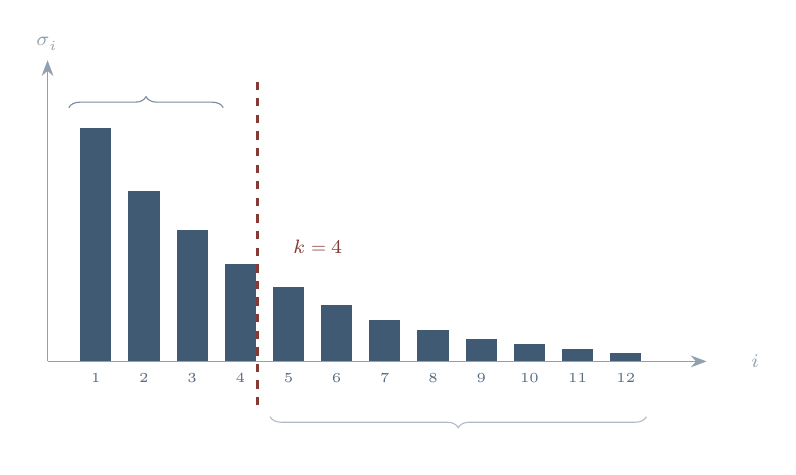
\begin{tikzpicture}[scale=0.9, >=Stealth]
  % 坐标轴
  \draw[->, navy!45, line width=0.6pt] (0,0)--(9.3,0) node[right,font=\scriptsize]{奇异值序号 $i$};
  \draw[->, navy!45, line width=0.6pt] (0,0)--(0,4.25) node[above,font=\scriptsize]{$\sigma_i$};
  % 柱子与刻度
  \foreach \i/\h in {1/3.30, 2/2.40, 3/1.85, 4/1.38, 5/1.05, 6/0.79,
                     7/0.59, 8/0.44, 9/0.32, 10/0.24, 11/0.17, 12/0.12}{
    \fill[navy!78] (\i*0.68-0.22,0) rectangle (\i*0.68+0.22,\h);
    \node[below,font=\tiny,text=navy!70] at (\i*0.68,-0.03) {\i};
  }
  % 截断线
  \draw[warnc, dashed, line width=0.9pt] (4*0.68+0.24,-0.62)--(4*0.68+0.24,4.05);
  \node[warnc, font=\scriptsize, anchor=west] at (4*0.68+0.36,1.62) {截断 $k=4$};
  % 保留括号（柱子上方）
  \draw[decorate, decoration={brace, amplitude=4pt}, navy!55]
      (0.3,3.58)--(4*0.68-0.24,3.58)
      node[midway, above=4pt, font=\tiny, text=navy] {保留};
  % 丢弃括号（刻度下方）
  \draw[decorate, decoration={brace, amplitude=4pt, mirror}, navy!32]
      (4*0.68+0.42,-0.78)--(8.45,-0.78)
      node[midway, below=4pt, font=\tiny, text=navy!60] {丢弃};
\end{tikzpicture}
\caption{一个典型的奇异值谱。奇异值快速衰减时，前几个分量就承载了绝大部分能量，
后面的“长尾”往往对应噪声或细节。$k$ 的选择就是在这个长尾上做截断。}
\label{fig:spectrum}
\end{figure}

图 \ref{fig:spectrum} 画出了一个典型的奇异值谱。真实的图像、文本、评分矩阵都有
类似的形状：少数几个奇异值很大，然后迅速掉进一个长尾。这正是低秩逼近能奏效的原因。

\begin{warnbox}[$k$ 不能看测试集来选]
在实际任务中，$k$ 是一个需要选择的超参数。常见做法有：取 $E(k)\ge0.95$ 的最小 $k$；
或者看谱图上的“肘部”；或者用交叉验证。但\textbf{绝不能}根据测试集上的表现来挑 $k$——
那等于用测试集训练，得到的评估结果会偏乐观。这是机器学习评估中最常见的错误之一。
\end{warnbox}

\subsection{一个算例：图像压缩}

设有一张 $512\times 512$ 的灰度图，把它看作矩阵 $A$。用 SVD 压缩的存储方案是：
只保留前 $k$ 个奇异值及对应的奇异向量，需要的存储量为
\begin{equation}
  \underbrace{k}_{\sigma_i}+\underbrace{512k}_{U_k}+\underbrace{512k}_{V_k}
  =k(1024+1)=1025k \quad\text{个数}.
\end{equation}
原图需要 $512^2=262144$ 个数。压缩比如下表所示。

\begin{table}[htbp]
\centering
\small
\caption{不同截断秩下的存储量与相对误差（$512\times512$ 图像）}\label{tab:compress}
\renewcommand{\arraystretch}{1.35}
\begin{tabular}{@{}ccccc@{}}
\toprule
$k$ & 存储量 & 占原图比例 & 压缩比 & 相对误差 $\nrm{A-A_k}_F/\nrm{A}_F$ \\
\midrule
$10$  & $10\,250$  & $3.9\%$  & $25.6:1$ & 依图像而定 \\
$30$  & $30\,750$  & $11.7\%$ & $8.5:1$  & 依图像而定 \\
$50$  & $51\,250$  & $19.6\%$ & $5.1:1$  & 依图像而定 \\
$100$ & $102\,500$ & $39.1\%$ & $2.6:1$  & 依图像而定 \\
$256$ & $262\,400$ & $100.1\%$& $1.0:1$  & 几乎为零 \\
\bottomrule
\end{tabular}
\end{table}

表 \ref{tab:compress} 里“相对误差”一列写了“依图像而定”，是因为它完全取决于图像的
奇异值谱，没有普适数值。对一张细节丰富的照片，$k=50$ 可能仍有可见的块状模糊；
对一张以大面积平滑区域为主的图像，$k=20$ 就可能看不出差别。

下面是用 NumPy 做这件事的代码，不到十行：

\begin{lstlisting}[language=Python]
import numpy as np
from numpy.linalg import svd

A = ...                            # 512 x 512 grayscale image, values in [0,1]
U, s, Vt = svd(A, full_matrices=False)   # economy (thin) SVD

def approx(U, s, Vt, k):
    return (U[:, :k] * s[:k]) @ Vt[:k]   # same as U_k @ diag(s_k) @ V_k.T

for k in (10, 30, 50, 100):
    Ak = approx(U, s, Vt, k)
    err = np.linalg.norm(A - Ak) / np.linalg.norm(A)
    print(f"k={k:3d}  relative error = {err:.4f}")
\end{lstlisting}

\begin{rem}
代码里 \texttt{U[:, :k] * s[:k]} 利用了 NumPy 的广播：形状 $(512,k)$ 的数组乘以形状
$(k,)$ 的数组，会按列逐列缩放。写成一个循环也完全可以，只是慢一些。
\end{rem}

\subsection{低秩逼近的局限}

Eckart--Young 定理很强，但它的适用范围有明确的边界，用错地方会得出误导性的结论。

\begin{enumerate}
  \item \textbf{“最佳”是相对于 F 范数和谱范数而言的。}如果误差的度量换成别的
        （例如逐元素绝对误差、加权误差、感知损失），$A_k$ 未必最优。
  \item \textbf{F 范数对大误差特别敏感。}因为误差是平方的，少数几个异常点就能主导
        整个目标。数据里有离群值时，SVD 低秩逼近会把它们“摊”到所有元素上，效果很差。
        这时应该用鲁棒 PCA 一类的方法。
  \item \textbf{缺失数据不能直接做 SVD。}推荐系统里的评分矩阵有大量空缺，而 SVD 要求
        矩阵完整。把缺失当成 $0$ 直接补全，会系统性地低估评分。正确做法是矩阵补全
        （matrix completion），它优化的是“只在已观测位置上”的误差，Eckart--Young
        定理在这里\textbf{不适用}。
  \item \textbf{计算成本随 $k$ 增长。}当 $k$ 接近 $\min(m,n)$ 时，截断 SVD 相对完整
        SVD 没有优势，还不如直接算。
\end{enumerate}

\begin{warnbox}[一个常见的误用]
有人把用户—物品评分矩阵的缺失项填 $0$，做 SVD，然后说“这就是协同过滤”。
这是错的：填 $0$ 相当于告诉算法“这个用户非常讨厌这部电影”，而事实上我们只是
不知道他的态度。这样的模型会把预测值整体压低，而且秩越低偏差越大。
正确的方法（如 FunkSVD、ALS）只对观测到的评分计算损失。
\end{warnbox}

\subsection*{自检}
\begin{enumerate}
  \item 若 $A$ 的奇异值为 $5,3,1$，写出 $\nrm{A-A_1}_2$、$\nrm{A-A_1}_F$ 与 $E(1)$。
  \item 证明：若 $\rank(A)=r$，则不存在秩小于 $r$ 的矩阵 $B$ 使 $\nrm{A-B}_F=0$。
  \item 为什么说“$A_k$ 同时是谱范数和 F 范数下的最优解”这件事并不显然？
        试构造一个反例说明：对一般的矩阵范数，两种意义下的最优解可能不同。
\end{enumerate}

% ============================================================
\section{伪逆与最小二乘}\label{sec:pinv}
% ============================================================

SVD 最早、最经典的用途之一，是求解“方程比未知数多”的最小二乘问题。
这一节说明为什么用 SVD 求解比用正规方程更可靠。

\subsection{超定方程为什么常常无解}

考虑线性方程组 $A\x=\bb$，其中 $A\in\R^{m\times n}$ 且 $m>n$（方程个数多于未知数）。
一般情况下，$\bb$ 不会恰好落在 $\Col(A)$ 里，方程组\textbf{无解}。

例如
\begin{equation}
  \begin{pmatrix}1&0\\0&1\\1&1\end{pmatrix}\begin{pmatrix}x_1\\x_2\end{pmatrix}
  =\begin{pmatrix}1\\1\\3\end{pmatrix}
\end{equation}
无解，因为前两个方程要求 $x_1=x_2=1$，代入第三个得 $2\neq3$。
三个方程在“争夺”两个未知数，不可能同时满足。

工程上的处理方式是退一步：不要求残差为零，只要求残差尽可能小。这就是最小二乘：
\begin{equation}\label{eq:ls}
  \x_{\mathrm{LS}}=\argmin_{\x\in\R^{n}}\nrm{A\x-\bb}_2^2 .
\end{equation}

\subsection{最小二乘的几何：把 b 投影到列空间}

$\nrm{A\x-\bb}_2^2$ 最小，等价于 $A\x$ 是 $\bb$ 在 $\Col(A)$ 上的\textbf{正交投影}。
理由很直观：如果 $A\x$ 不是投影点，那么沿着 $\Col(A)$ 内的方向微调 $\x$，还能让距离更小。

于是可以写 $\bb=A\x+\mathbf{e}$，其中 $\mathbf{e}\perp\Col(A)$，即 $A\T\mathbf{e}=\mathbf{0}$。
两边左乘 $A\T$：
\begin{equation}
  A\T\bb=A\T A\x+A\T\mathbf{e}=A\T A\x .
\end{equation}
这就是著名的\textbf{正规方程}（normal equation）。

\begin{thm}\label{thm:normal-eq}
若 $A$ 列满秩（$\rank(A)=n$），则 $A\T A$ 可逆，最小二乘问题 \eqref{eq:ls} 有唯一解
\begin{equation}
  \x_{\mathrm{LS}}=(A\T A)^{-1}A\T\bb .
\end{equation}
\end{thm}

\begin{proof}
$A\T A$ 可逆性由命题 \ref{prop:ata-psd}：若 $A$ 列满秩，则 $\Null(A)=\{\mathbf{0}\}$，
故 $\Null(A\T A)=\{\mathbf{0}\}$，$n$ 阶方阵满秩。
唯一性：目标函数是严格凸二次函数
$f(\x)=\x\T A\T A\x-2\bb\T A\x+\bb\T\bb$，其 Hessian $2A\T A$ 正定，
唯一的驻点就是全局最小点。令梯度为零即得正规方程。
\end{proof}

\subsection{伪逆：把逆推广到所有矩阵}

方阵可逆时 $\x=A^{-1}\bb$；可逆性不成立时，我们希望有一个“替代品”，
它在可逆的情形下退化为逆，在不可逆或非方阵时仍然给出合理的结果。

\begin{defn}[Moore--Penrose 伪逆]\label{def:pinv}
设 $A=U\Sigma V\T$ 是 $A\in\R^{m\times n}$ 的 SVD，$\rank(A)=r$。定义
\begin{equation}
  A^{+}=V\Sigma^{+}U\T,\qquad
  \Sigma^{+}=\diag\Big(\frac{1}{\sigma_1},\dots,\frac{1}{\sigma_r},0,\dots,0\Big)\in\R^{n\times m},
\end{equation}
称 $A^{+}$ 为 $A$ 的\textbf{伪逆}（pseudoinverse）。
\end{defn}

也就是说：把非零奇异值取倒数，再转置一下位置。

\begin{prop}[伪逆的基本性质]\label{prop:pinv-prop}

\begin{enumerate}
  \item 若 $A$ 可逆，则 $A^{+}=A^{-1}$；
  \item $AA^{+}A=A$，$A^{+}AA^{+}=A^{+}$；
  \item $AA^{+}$ 是到 $\Col(A)$ 的正交投影，$A^{+}A$ 是到 $\Row(A)$ 的正交投影；
  \item $\rank(A^{+})=\rank(A)$。
\end{enumerate}
\end{prop}

\begin{proof}
(1) 若 $A$ 可逆，则 $m=n=r$，$\Sigma$ 与 $\Sigma^{+}$ 互为逆，
故 $A^{+}=V\Sigma^{-1}U\T=(U\Sigma V\T)^{-1}=A^{-1}$。

(3) $AA^{+}=U\Sigma\Sigma^{+}U\T$，而 $\Sigma\Sigma^{+}$ 是对角元前 $r$ 个为 $1$、
其余为 $0$ 的 $m$ 阶对角阵，故 $AA^{+}=U_rU_r\T$，正是到
$\Span\{\bu_1,\dots,\bu_r\}=\Col(A)$ 的投影。同理 $A^{+}A=V_rV_r\T$。

(2)(4) 直接由定义验证。
\end{proof}

\begin{thm}[最小二乘的伪逆解]\label{thm:pinv-ls}
对任意 $A\in\R^{m\times n}$ 与 $\bb\in\R^{m}$，$\x=A^{+}\bb$ 是问题 \eqref{eq:ls} 的
\textbf{极小范数最小二乘解}：它使残差最小，且在所有达到最小残差的解中，它的范数最小。
若 $A$ 列满秩，则它就是唯一的最小二乘解。
\end{thm}

\begin{proof}[证明要点]
把 $\bb$ 按 $U$ 的列分解：$\bb=\sum_{i=1}^{m}c_i\bu_i$，其中 $c_i=\bu_i\T\bb$。
对任意 $\x$，写 $\x=\sum_{j=1}^{n}d_j\vv_j$，则
\begin{equation}
  A\x=\sum_{j=1}^{r}\sigma_jd_j\bu_j,\qquad
  \nrm{A\x-\bb}_2^2=\sum_{j=1}^{r}(\sigma_jd_j-c_j)^2+\sum_{i=r+1}^{m}c_i^2 .
\end{equation}
第二项与 $\x$ 无关，是第一项可以取到 $0$，只要 $d_j=c_j/\sigma_j$（$j\le r$）。
于是所有最小二乘解都有形式
$\x=\sum_{j=1}^{r}\frac{c_j}{\sigma_j}\vv_j+\sum_{j=r+1}^{n}d_j\vv_j$，
而后半部分的系数 $d_j$ 任意。显然取 $d_j=0$ 时 $\nrm{\x}_2$ 最小。
这正是 $A^{+}\bb$ 的展开式。
\end{proof}

\begin{keybox}[伪逆解的展开式]
\begin{equation*}
  A^{+}\bb=\sum_{i=1}^{r}\frac{\bu_i\T\bb}{\sigma_i}\,\vv_i .
\end{equation*}
每一项是“$\bb$ 在第 $i$ 个左奇异方向上的投影系数，除以 $\sigma_i$，
再放到第 $i$ 个右奇异方向上”。$\sigma_i$ 越小，这一项被放大得越厉害——
这正是病态问题的来源，也是后面要截断的原因。
\end{keybox}

\subsection{为什么不用正规方程}

从数学上看，$(A\T A)^{-1}A\T\bb$ 与 $A^{+}\bb$ 在精确算术下是同一个东西。
但在浮点数下，两者的表现可能天差地别。

\begin{prop}[误差放大]\label{prop:cond-error}
设 $A$ 列满秩，$\bb$ 有扰动 $\delta\bb$，解相应变为 $\x+\delta\x$。则
\begin{equation}
  \frac{\nrm{\delta\x}_2}{\nrm{\x}_2}\le\kappa(A)\cdot
  \frac{\nrm{\delta\bb}_2}{\nrm{\bb}_2} .
\end{equation}
若改用正规方程求解，扰动会被放大 $\kappa(A\T A)=\kappa(A)^2$ 倍。
\end{prop}

\begin{proof}
由 $\x=A^{+}\bb$ 得 $\delta\x=A^{+}\delta\bb$，故
$\nrm{\delta\x}\le\nrm{A^{+}}_2\nrm{\delta\bb}=\frac{1}{\sigma_r}\nrm{\delta\bb}$。
又 $\nrm{\bb}=\nrm{A\x}\le\sigma_1\nrm{\x}$，即 $\nrm{\x}\ge\nrm{\bb}/\sigma_1$。
两式相除即得。正规方程部分由 $\kappa(A\T A)=\kappa(A)^2$（命题 \ref{prop:cond-square}）。
\end{proof}

\begin{insight}[条件数的平方为什么致命]
双精度浮点有大约 $16$ 位十进制有效数字。若 $\kappa(A)=10^{8}$，用 SVD 求解还剩约
$8$ 位可信；用正规方程则放大到 $10^{16}$，结果可能\textbf{一位有效数字都不剩}。
更糟的是，$A\T A$ 在计算过程中会丢失信息：原本不同的小奇异值，平方之后可能
小于舍入误差，被直接抹成零，矩阵的秩看起来就变了。
\end{insight}

\begin{warnbox}[实践建议]
解最小二乘时，优先用 \texttt{np.linalg.lstsq}（内部用 SVD 或 QR），
而不是自己写 \texttt{inv(A.T @ A) @ A.T @ b}。
后者在 $A$ 病态时会给出完全错误的结果，而且不报任何错。
判断是否需要担心：先算一下 \texttt{np.linalg.cond(A)}，
若超过 $10^{8}$ 就要警惕，超过 $10^{12}$ 基本不能用。
\end{warnbox}

\subsection{截断 SVD 与正则化}

病态问题的根源是那些很小的奇异值：它们对应的项
$(\bu_i\T\bb/\sigma_i)\vv_i$ 被放大了 $1/\sigma_i$ 倍，噪声因此被放大成灾。

最直接的处理是\textbf{截断}：只保留前 $k$ 个奇异值，
\begin{equation}
  \x_k=\sum_{i=1}^{k}\frac{\bu_i\T\bb}{\sigma_i}\vv_i .
\end{equation}
这相当于假设“$\bb$ 在小奇异方向上的分量都是噪声”。

另一种更平滑的做法是\textbf{岭回归}（Tikhonov 正则化）：
\begin{equation}\label{eq:ridge}
  \x_{\lambda}=\argmin_{\x}\nrm{A\x-\bb}_2^2+\lambda\nrm{\x}_2^2
  =\sum_{i=1}^{r}\frac{\sigma_i}{\sigma_i^2+\lambda}\,(\bu_i\T\bb)\,\vv_i ,
\end{equation}
其中 $\lambda>0$ 是正则化强度。注意过滤因子
$\frac{\sigma_i}{\sigma_i^2+\lambda}$ 的行为：当 $\sigma_i\gg\sqrt{\lambda}$ 时它接近
$1/\sigma_i$（几乎不改变），当 $\sigma_i\ll\sqrt{\lambda}$ 时它接近 $\sigma_i/\lambda$
（强烈压制）。

\begin{figure}[htbp]
\centering
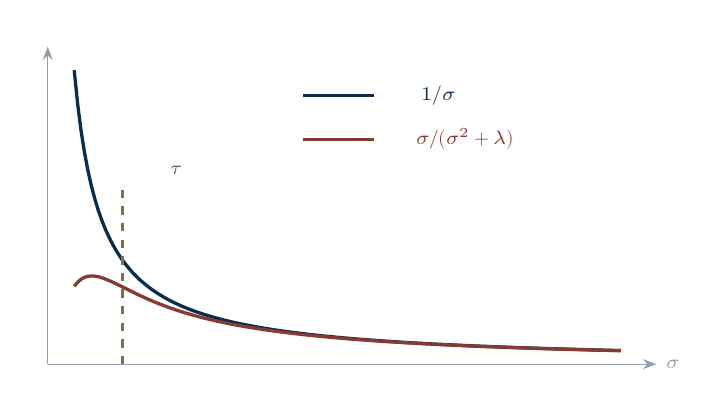
\begin{tikzpicture}[scale=1.12, >=Stealth]
  % 坐标轴
  \draw[->, navy!45] (0,0)--(6.9,0) node[right,font=\scriptsize]{$\sigma$};
  \draw[->, navy!45] (0,0)--(0,3.6) node[above,font=\scriptsize]{过滤因子};
  % 无正则化 1/sigma
  \draw[navy, line width=1.2pt, domain=0.30:6.5, samples=160]
      plot (\x, {1.0/\x});
  % 岭回归
  \draw[warnc, line width=1.2pt, domain=0.30:6.5, samples=200]
      plot (\x, {\x/(\x*\x+0.25)});
  % 截断阈值
  \draw[gold!80!black, dashed, line width=1pt] (0.85,0)--(0.85,2.05);
  \node[gold!70!black, font=\scriptsize, anchor=west, align=left]
      at (0.95,2.20) {截断阈值 $\tau$};
  % 图例
  \draw[navy, line width=1.2pt] (2.9,3.05)--(3.7,3.05);
  \node[navy, font=\scriptsize, anchor=west] at (3.8,3.05) {无正则化 $1/\sigma$};
  \draw[warnc, line width=1.2pt] (2.9,2.55)--(3.7,2.55);
  \node[warnc, font=\scriptsize, anchor=west] at (3.8,2.55) {岭回归 $\sigma/(\sigma^{2}+\lambda)$};
\end{tikzpicture}
\caption{三种处理小奇异值的方式。截断（虚线）是“保留或丢弃”的硬开关；
岭回归（红色）是平滑的过渡，在 $\sigma\approx\sqrt{\lambda}$ 附近开始压制；
无正则化（深蓝）在 $\sigma\to0$ 时发散。}
\label{fig:filter}
\end{figure}

图 \ref{fig:filter} 画出了三种策略的差异。截断简单但会引入不连续；岭回归平滑，
代价是需要选择 $\lambda$。两者都是“用一点偏差换取大量方差 reduction”的典型例子，
这正是机器学习中偏差—方差权衡的具体形态。

\subsection*{自检}
\begin{enumerate}
  \item 对 $A=\bigl(\begin{smallmatrix}1&1\\1&1\\0&0\end{smallmatrix}\bigr)$ 与 $\bb=(2,2,1)\T$，
        求 $A^{+}\bb$ 与残差。
  \item 证明 $AA^{+}$ 是对称矩阵，且 $(AA^{+})^2=AA^{+}$（即它是投影矩阵）。
  \item 若 $\lambda\to0$，式 \eqref{eq:ridge} 退化成什么？若 $\lambda\to\infty$ 呢？
\end{enumerate}

% ============================================================
\section{SVD 与主成分分析}\label{sec:pca}
% ============================================================

主成分分析（PCA）是数据科学中使用最广的降维方法，而它与 SVD 的关系简单到令人意外：
\textbf{PCA 就是对中心化后的数据矩阵做 SVD}。理解这一点，可以避免很多误用。

\subsection{PCA 想解决什么问题}

设数据矩阵 $X\in\R^{N\times D}$，$N$ 个样本、$D$ 个特征，第 $i$ 行是第 $i$ 个样本。
当 $D$ 很大时，我们想找 $k\ll D$ 个新方向，把数据投影上去，使投影后的点
尽量分散（保留最多的变异），同时尽量保持样本之间的相对距离。

“分散”用方差度量。所以问题可以写成：找一个单位向量 $\mathbf{p}_1$，
使 $\nrm{X\mathbf{p}_1}_2^2$ 最大。

\subsection{第一步：中心化}

注意：PCA 要求数据\textbf{已经中心化}，即每一列的均值为零。若不中心化，
第一主成分会指向数据的均值方向，而不是变异最大的方向（详见 \ref{sec:no-center} 节）。

设中心化后的矩阵仍记为 $X$，则样本协方差矩阵为
\begin{equation}
  S=\frac{1}{N-1}X\T X\in\R^{D\times D} .
\end{equation}

\subsection{第二步：对 X 做 SVD}

设 $X=U\Sigma V\T$，其中 $U\in\R^{N\times r}$、$\Sigma\in\R^{r\times r}$、
$V\in\R^{D\times r}$（$r=\rank(X)$，通常 $r=\min(N-1,D)$）。则
\begin{equation}
  S=\frac{1}{N-1}X\T X=\frac{1}{N-1}V\Sigma^2V\T .
\end{equation}
与协方差矩阵的特征分解 $S=Q\Lambda Q\T$ 对比，立刻得到：
\begin{itemize}
  \item \textbf{主成分方向}是 $V$ 的列，即 $X$ 的右奇异向量；
  \item \textbf{第 $j$ 个主成分的方差}是 $\sigma_j^2/(N-1)$；
  \item \textbf{主成分得分}（每个样本在新坐标下的坐标）是 $U\Sigma$ 的列。
\end{itemize}

\begin{thm}[PCA 与 SVD 的等价性]\label{thm:pca-svd}
对中心化矩阵 $X$，其前 $k$ 个主成分方向等于 $X$ 的前 $k$ 个右奇异向量，
前 $k$ 个主成分的方差之和等于 $\sum_{j=1}^{k}\sigma_j^2/(N-1)$，且
\begin{equation}
  \text{累计解释方差比例}=\frac{\sum_{j=1}^{k}\sigma_j^2}{\sum_{j=1}^{r}\sigma_j^2}=E(k),
\end{equation}
与式 \eqref{eq:energy} 定义的“能量比例”完全一致。
\end{thm}

这个定理说明：PCA 与低秩逼近是同一件事的两个说法。用主成分做降维后重构，
得到的就是 $X_k=U_k\Sigma_kV_k\T$，而它正是 $X$ 的最佳秩 $k$ 逼近。

\begin{insight}[为什么可以直接对 X 做 SVD，而不必算协方差矩阵]
计算 $D\times D$ 的协方差矩阵需要 $O(ND^2)$ 次运算，还需要 $O(D^2)$ 的存储；
当 $D=10^4$ 时，$S$ 有 $10^8$ 个元素。而直接对 $X$ 做 SVD（用第 \ref{sec:compute}
节的方法）可以只算前 $k$ 个奇异三元组，代价是 $O(NDk)$。
更重要的是：构造 $S=X\T X$ 会把条件数平方，细小的方差方向会被数值误差吞掉。
\end{insight}

\subsection{第三步：解释方差与选择主成分个数}

实践中常画“累计解释方差曲线”，选一个拐点。例如前 $k$ 个主成分解释了 $95\%$ 的方差，
就可以认为降到 $k$ 维是合理的。

\begin{rem}
“解释 $95\%$ 的方差”不等于“保留了 $95\%$ 的信息”。方差只刻画二阶统计量，
如果数据的结构体现在高阶矩上（例如明显的聚类），低方差方向也可能含有分类所需的信息。
PCA 是无监督的，它不知道你后面要做什么任务。
\end{rem}

\subsection{不中心化会发生什么}\label{sec:no-center}

\begin{exam}\label{exam:no-center}
设 $N=100$ 个二维样本，全部集中在 $(100,100)$ 附近，坐标的标准差为 $1$。
数据大致是各向同性的（两个方向变异差不多）。

\textbf{中心化后}：均值为 $0$，协方差近似为 $I$，两个主成分方向任意（退化情形），
解释方差各占一半。

\textbf{不中心化}：数据的均值本身是 $(100,100)$，其范数约为 $141$，
远远大于波动幅度 $1$。此时 $X\T X$ 被均值项主导：
\begin{equation}
  X\T X=\sum_{i=1}^{N}\x_i\x_i\T\approx N\,\boldsymbol{\mu}\boldsymbol{\mu}\T+N\,S ,
\end{equation}
第一项的特征值约为 $N\nrm{\boldsymbol{\mu}}^2\approx100\times20000=2\times10^{6}$，
第二项只有 $N\approx100$。于是第一主成分几乎正好是 $\boldsymbol{\mu}/\nrm{\boldsymbol{\mu}}
=(1,1)\T/\sqrt2$ 方向——它指向原点，而不是数据变异最大的方向。
\end{exam}

这个例子说明：\textbf{不中心化的 PCA 得到的第一主成分，主要反映“数据离原点有多远”，
而不是“数据在哪个方向上变化最大”}。对图像数据尤其要注意：像素值都是正数，
不中心化时第一主成分往往就是“平均亮度”。

\begin{warnbox}[两个常见错误]
\textbf{错误一}：把未中心化的矩阵直接做 SVD，然后称之为 PCA。
这在数学上仍然是 SVD，但不是 PCA——它对应的是“未中心化的主成分分析”，
解释的是均方值而非方差。

\textbf{错误二}：对已经中心化的数据再做一次标准化（除以标准差）却不说明。
标准化会改变各特征的权重，得到的其实是“相关矩阵的 PCA”，
与“协方差矩阵的 PCA”结果不同。两者没有对错，但必须写清楚。
\end{warnbox}

\subsection*{自检}
\begin{enumerate}
  \item 若 $X$ 已中心化且 $N=50$，前两个奇异值为 $10$ 和 $5$，
        求前两个主成分的方差与累计解释比例。
  \item 为什么 $X$ 的秩最多是 $\min(N-1,D)$（在中心化之后）？
  \item 如果把 PCA 的结果用于分类，选择 $k$ 时应该看解释方差还是看分类准确率？
        两者的区别是什么？
\end{enumerate}

% ============================================================
\section{怎么算：从双对角化到随机化算法}\label{sec:compute}
% ============================================================

前面的定义和定理都是“数学上存在”，实际问题还要考虑“算得动、算得准”。
这一节介绍三条主流路线，重点不在实现细节，而在\textbf{什么时候该用哪一条}。

\subsection{为什么不能直接对 A 转置乘 A 求特征值}

由第 \ref{sec:exist} 节的构造，最“自然”的算法是：算 $A\T A$，求它的特征分解，
开平方得奇异值。这个算法在数学上完全正确，在数值上却很糟糕。

\begin{exam}
设 $A$ 的奇异值为 $1$ 与 $10^{-8}$。双精度下，$A\T A$ 的特征值是 $1$ 与 $10^{-16}$。
而 $1$ 的浮点表示本身就有约 $10^{-16}$ 的相对误差，计算 $A\T A$ 的过程中还会
引入新的舍入误差。结果是：$10^{-16}$ 这个特征值完全被误差淹没，
甚至可能算出负数，开平方直接失败。

用 SVD 直接算，$10^{-8}$ 与 $1$ 相差 $8$ 个数量级，在双精度下可以清楚分辨。
\end{exam}

一般地，若 $\kappa(A)=10^{k}$，则 $\kappa(A\T A)=10^{2k}$。
$k=8$ 时 $\kappa(A\T A)=10^{16}$，已经超出双精度的分辨能力。
这就是为什么所有主流库（LAPACK、NumPy、MATLAB）都用专门的双对角化算法，
而不是“特征值 + 开方”。

\subsection{Golub--Kahan 双对角化}

这是 LAPACK 中 \texttt{gesdd} 的核心思路，分两步：

\begin{enumerate}
  \item \textbf{双对角化}：用 Householder 变换从左右两侧交替作用，把 $A$ 化成
        只有主对角线和超对角线非零的“双对角矩阵” $B$：
        \begin{equation}
          A=P\,B\,Q\T,\qquad
          B=\begin{pmatrix}
          d_1&e_1&&\\
          &d_2&e_2&\\
          &&\ddots&\ddots\\
          &&&d_n
          \end{pmatrix}.
        \end{equation}
        这一步是有限步的，不引入迭代误差，代价 $O(mn^2)$。
  \item \textbf{对 $B$ 做隐式 QR 迭代}：$B$ 是稀疏的，QR 迭代可以保持双对角结构，
        每次迭代只需 $O(n)$ 的代价。收敛后得到 $B$ 的 SVD，再与 $P,Q$ 合并。
\end{enumerate}

整体复杂度为 $O(mn^2)$（$m\ge n$），这是稠密矩阵 SVD 的标准代价。

\subsection{幂迭代：只要最大的那一个}

如果只需要最大的奇异值（以及对应的向量），没必要做完整分解。
幂迭代利用一个简单的事实：反复用 $A\T A$ 作用，最大特征值方向会逐渐占主导。

\begin{lstlisting}[language=Python]
import numpy as np

def power_svd(A, iters=500, tol=1e-10):
    n = A.shape[1]
    v = np.random.randn(n); v /= np.linalg.norm(v)
    sigma_old = 0.0
    for _ in range(iters):
        w = A.T @ (A @ v)          # same as A.T @ A @ v
        sigma = np.linalg.norm(w)  # sqrt of Rayleigh quotient
        v = w / sigma
        if abs(sigma - sigma_old) < tol * sigma:
            break
        sigma_old = sigma
    u = (A @ v) / sigma
    return sigma, u, v
\end{lstlisting}

收敛速度由奇异值之比决定：误差每步乘以 $(\sigma_2/\sigma_1)^2$。
若 $\sigma_2/\sigma_1=0.9$，需要约 $200$ 步才能把误差降到 $10^{-9}$；
若比值是 $0.5$，十几步就够了。\textbf{奇异值衰减越快，幂迭代越快}——
这与“低秩矩阵容易处理”的直觉一致。

\begin{rem}
幂迭代的收敛速度依赖谱间隙 $\sigma_1-\sigma_2$。若前两个奇异值非常接近，
它会很慢。此时可以用“块幂迭代”（同时迭代多个向量）或 Lanczos 方法。
实际库中的 \texttt{svds}（SciPy）用的是 Lanczos/Arnoldi，通常比朴素幂迭代快得多。
\end{rem}

\subsection{随机化 SVD：用随机投影找列空间}

当矩阵非常大（比如 $10^6\times10^5$）却又近似低秩时，可以只算前 $k$ 个分量。
随机化算法由 Halko、Martinsson 与 Tropp 在 2011 年系统化，思路出奇地简单：

\begin{enumerate}
  \item 生成一个 $n\times(k+p)$ 的随机矩阵 $\Omega$（$p$ 是过采样参数，常取 $5\sim10$），
        元素独立取自标准正态分布；
  \item 计算 $Y=A\Omega$。这是一个“随机投影”，它把 $A$ 的列空间压缩到
        $k+p$ 维，大概率保留了主要方向；
  \item 对 $Y$ 做 QR 分解 $Y=QR$，$Q$ 的列是 $\Col(A)$ 的近似标准正交基；
  \item 计算小矩阵 $B=Q\T A$（尺寸 $(k+p)\times n$），对它做标准 SVD：
        $B=\tilde{U}\Sigma V\T$；
  \item 令 $U=Q\tilde{U}$，得到 $A\approx U\Sigma V\T$。
\end{enumerate}

关键在于第 4 步：真正的 SVD 只作用在一个 $(k+p)\times n$ 的小矩阵上，
代价从 $O(mn^2)$ 降到 $O(mn(k+p))$。当 $k\ll n$ 时，这是数量级的加速。

\begin{keybox}[随机化算法的代价与保证]
代价：$O(mn\log k + (m+n)k^2)$，主要是两次矩阵乘法。
保证：误差满足
$\nrm{A-U\Sigma V\T}_2\le\big(1+O(1)\big)\sigma_{k+1}$（以高概率），
即与最佳秩 $k$ 逼近同阶。代价是“高概率”而非“一定”——
随机算法总有小概率失败，实践中靠过采样 $p$ 把失败概率压到极低。
\end{keybox}

\subsection{该选哪条路线}

\begin{table}[htbp]
\centering
\small
\caption{不同场景下的方法选择}\label{tab:methods}
\renewcommand{\arraystretch}{1.35}
\begin{tabular}{@{}>{\raggedright\arraybackslash}p{3.4cm}>{\raggedright\arraybackslash}p{2.6cm}>{\raggedright\arraybackslash}p{5.2cm}>{\raggedright\arraybackslash}p{3.2cm}@{}}
\toprule
\textbf{场景} & \textbf{矩阵规模} & \textbf{推荐方法} & \textbf{复杂度} \\
\midrule
稠密、需要全部奇异值 & $10^3$ 以内 & LAPACK 双对角化（\texttt{np.linalg.svd}） & $O(mn^2)$ \\
稠密、只要前 $k$ 个 & $10^3\sim10^4$ & 截断 SVD（\texttt{scipy.sparse.linalg.svds}） & $O(mnk)$ \\
稀疏、超大 & $10^6$ 以上 & Lanczos / 随机化 SVD & $O(mnk)$ \\
只要最大奇异值 & 任意 & 幂迭代 & $O(mn)$/步 \\
在线、数据流 & 任意 & 增量 SVD 或随机化 & 视实现 \\
\bottomrule
\end{tabular}
\end{table}

\begin{warnbox}[稀疏矩阵的陷阱]
对稀疏矩阵做完整 SVD，得到的 $U$ 和 $V$ 几乎一定是稠密的。若原矩阵有 $10^8$
个非零元，而 $U$ 是 $10^6\times10^6$ 的稠密矩阵，存储直接爆掉（$8$ 字节 $\times10^{12}$）。
这时必须只算前 $k$ 个分量，并且用不显式存储 $U$ 全体的接口。
\end{warnbox}

\subsection*{自检}
\begin{enumerate}
  \item 若 $\sigma_1=1$、$\sigma_2=0.99$，幂迭代要把误差降到 $10^{-6}$ 需要多少步？
  \item 为什么随机化 SVD 要过采样（取 $k+p$ 而不是正好 $k$）？
  \item 对一个 $10000\times100$ 的矩阵，完整 SVD 与只算前 $10$ 个奇异值，
        代价大约相差多少倍？
\end{enumerate}

% ============================================================
\section{应用案例}\label{sec:app}
% ============================================================

这一节把前面所有工具串起来，看几个真实场景里 SVD 是怎么用的。
每个案例都强调同一件事：\textbf{先把问题翻译成“低秩 + 某个损失函数”，再决定用不用 SVD}。

\subsection{图像压缩}

原理已在第 \ref{sec:lowrank} 节说明：把图像看作矩阵，截断 SVD 保留前 $k$ 个分量。
这里补充两个实践细节。

\textbf{分块处理。}对自然图像，整图 SVD 的效果往往不如分成 $8\times8$ 或 $16\times16$
的小块分别做 SVD 再拼回去。原因是局部块的相关性更强、奇异值衰减更快，
同样的 $k$ 能保留更多能量。JPEG 用的 DCT 本质上也是这个思路。

\textbf{彩色图像。}对 RGB 三个通道分别做 SVD，或者先把图像转到 YCbCr 空间，
对人眼不敏感的两个色度通道做更激进的截断。后者是 JPEG 的标准做法。

\subsection{推荐系统：潜在因子模型}

设评分矩阵 $R\in\R^{M\times N}$，$M$ 个用户、$N$ 个物品，大部分元素缺失。
假设用户的偏好由 $k$ 个潜在因子决定，即
\begin{equation}
  R_{ui}\approx \mathbf{p}_u\T\mathbf{q}_i ,
\end{equation}
其中 $\mathbf{p}_u,\mathbf{q}_i\in\R^{k}$。用矩阵语言，就是 $R\approx PQ\T$，
$P\in\R^{M\times k}$，$Q\in\R^{N\times k}$，即 $R$ 近似秩 $k$。

如果 $R$ 是完整的，直接做截断 SVD 就得到最优的 $P,Q$（在 F 范数下）。
但 $R$ 有大量缺失，Eckart--Young 定理不适用——我们只能最小化
\begin{equation}
  \min_{P,Q}\sum_{(u,i)\in\Omega}\big(R_{ui}-\mathbf{p}_u\T\mathbf{q}_i\big)^2
  +\lambda\big(\nrm{P}_F^2+\nrm{Q}_F^2\big),
\end{equation}
其中 $\Omega$ 是观测到的评分集合。这需要用交替最小二乘（ALS）或随机梯度下降求解，
不能直接调用 SVD。

\begin{rem}
Netflix Prize（2006--2009）让这类方法广为人知。获胜方案并非纯 SVD，
而是上百个模型的集成，但其中的核心组件确实是带正则化的矩阵分解。
这个案例的教训是：\textbf{模型结构比单一算法的精妙更重要}。
\end{rem}

\subsection{潜在语义分析}

文档—词频矩阵 $X\in\R^{D\times V}$（$D$ 篇文档、$V$ 个词）极其稀疏且高维。
直接用它算相似度，会遇到“同义词不匹配”的问题：查“汽车”找不到写着“轿车”的文档。

潜在语义分析（LSA）的做法是：对 $X$ 做截断 SVD，$X\approx U_k\Sigma_kV_k\T$，
然后用 $U_k\Sigma_k$ 的第 $i$ 行作为第 $i$ 篇文档的 $k$ 维表示。
在这个低维空间里，“汽车”和“轿车”因为经常出现在相似的文档中，
会有相近的坐标，相似度自然就高了。

这一步的实质是：\textbf{把“词—文档”共现关系压缩成 $k$ 个潜在主题}，
每个奇异向量对应一个主题，奇异值表示该主题的重要性。

\subsection{降噪与信号分离}

若观测矩阵 $Y=A+E$，其中 $A$ 低秩（真实信号）、$E$ 是随机噪声（满秩但奇异值小），
则截断 SVD 可以近似恢复 $A$：
\begin{equation}
  \hat{A}=Y_k\approx A .
\end{equation}
噪声的奇异值分布通常比较均匀（没有明显的“大奇异值”），而信号的能量集中在少数几个
方向上，两者在谱上分得开。这就是“奇异值谱上的信噪分离”。

\begin{warnbox}[降噪的边界]
这个论证成立的前提是“信号低秩、噪声不低秩，且信号能量占优”。
若噪声本身有结构（例如周期性条纹、固定的背景纹理），它的奇异值也可能很大，
截断反而会保留噪声、丢掉信号。用之前先看一眼奇异值谱，不要盲信。
\end{warnbox}

\subsection{其他值得一提的应用}

\begin{itemize}
  \item \textbf{线性回归的正则化}：岭回归、主成分回归都建立在 SVD 之上
        （见式 \eqref{eq:ridge}）。
  \item \textbf{模型压缩}：把神经网络的大权重矩阵做低秩分解，减少参数量与计算量。
  \item \textbf{控制与系统辨识}：用 SVD 做平衡截断（balanced truncation），
        把高维动力系统降阶。
  \item \textbf{计算几何}：点云的主方向分析、平面拟合，本质都是对协方差矩阵做特征分解，
        也就是对数据矩阵做 SVD。
\end{itemize}

\subsection*{自检}
\begin{enumerate}
  \item 为什么推荐系统不能直接对评分矩阵做 SVD？把缺失值填 $0$ 会带来什么偏差？
  \item LSA 中，$U_k\Sigma_k$ 与 $V_k$ 分别代表什么？为什么用 $U_k\Sigma_k$ 而不是 $U_k$？
  \item 若噪声的奇异值也很大，截断 SVD 降噪会失败。举一个具体的例子。
\end{enumerate}

% ============================================================
\section{十个常见误区}\label{sec:pitfall}
% ============================================================

这一节收集了教学中反复出现的误解。每一条都给出正确说法与理由，
建议逐条对照自己的理解检查一遍。

\begin{enumerate}[leftmargin=2.2em, itemsep=0.9em]

  \item \textbf{“SVD 就是对方阵做特征值分解。”}

  \textbf{不对。}特征值分解要求矩阵是方阵，而且即使方阵也可能不可对角化
  （例如 $\bigl(\begin{smallmatrix}1&1\\0&1\end{smallmatrix}\bigr)$）；有特征值时还可能涉及复数。
  SVD 对\textbf{任意} $m\times n$ 实矩阵都存在，且只用到正交矩阵与实数，
  条件宽松得多。二者的联系是：SVD 是 $A\T A$ 的特征分解“开平方”的产物，
  但 SVD 本身作用在 $A$ 上。

  \item \textbf{“奇异值可以是负数。”}

  \textbf{不对。}奇异值定义为 $\sigma_i=\sqrt{\lambda_i(A\T A)}$，取的是非负平方根。
  特征值可以为负、为复数，奇异值永远 $\ge0$。
  这就是为什么对称矩阵满足 $\sigma_i=\abs{\lambda_i}$ 而不是 $\sigma_i=\lambda_i$。

  \item \textbf{“一个矩阵的 SVD 是唯一的。”}

  \textbf{部分对，部分不对。}奇异值唯一；奇异向量在单重奇异值时唯一到符号，
  在重奇异值时只有子空间唯一。所以不同软件算出的 $\bu_i$ 可能差一个负号，
  甚至（重根时）差一个正交旋转。比较两组结果时，要比较
  $\abs{\bu_i\T\hat{\bu}_i}$ 或投影矩阵，而不是逐元素比较。

  \item \textbf{“算 SVD 就是算 $A\T A$ 的特征值再开方。”}

  \textbf{数学上对，工程上错。}$\kappa(A\T A)=\kappa(A)^2$，构造 $A\T A$ 会让
  条件数平方。$\kappa(A)=10^{8}$ 时，$A\T A$ 的条件数达到 $10^{16}$，
  双精度下小奇异值完全丢失。实际库用的是双对角化加 QR 迭代（第 \ref{sec:compute} 节）。

  \item \textbf{“$\sigma$ 就是标准差。”}

  \textbf{看语境。}在 SVD 里 $\sigma_i$ 是奇异值；在统计里 $\sigma$ 是标准差、
  $\sigma^2$ 是方差。本讲义用 $s^2$ 或 $\mathrm{Var}$ 表示方差以避免混淆。
  读论文时若看到 $\sigma_i^2$，要先确认它是“奇异值的平方”还是“方差”。

  \item \textbf{“对数据矩阵做 SVD 就是 PCA。”}

  \textbf{少了关键一步：中心化。}未中心化的 SVD 分解的是“均方值”而不是“方差”，
  第一主成分会指向均值方向（例 \ref{exam:no-center}）。
  对图像数据尤其明显：像素非负，不中心化时第一主成分几乎就是平均亮度图。

  \item \textbf{“截断秩 $k$ 用测试集上的效果来选。”}

  \textbf{绝对不行。}这等于用测试集调参，评估结果会系统性偏乐观。
  正确做法是用训练集/验证集选 $k$，测试集只在最后用一次；
  或者用解释方差、谱图肘部等不依赖标签的准则。

  \item \textbf{“稀疏矩阵也能直接做 SVD，反正库会处理。”}

  \textbf{能算，但存不下。}稀疏矩阵的 $U$、$V$ 通常是稠密的。
  $10^6\times10^6$ 的稠密矩阵需要 $8$\,TB（双精度），直接爆内存。
  必须用只返回前 $k$ 个分量的接口（如 \texttt{svds}），
  并清楚 $U_k$ 仍可能是 $10^6\times k$ 的稠密矩阵。

  \item \textbf{“截断 SVD 是所有意义下的最优低秩逼近。”}

  \textbf{只在谱范数与 F 范数下最优}（Eckart--Young 定理）。
  若损失函数换成逐元素绝对误差、加权误差、或“只在观测位置上计算”的误差
  （推荐系统的情形），$A_k$ 未必最优，甚至可能很糟。
  用之前先确认损失函数与定理匹配。

  \item \textbf{“求伪逆时直接用 $1/\sigma_i$ 就行。”}

  \textbf{要截断。}当 $\sigma_i$ 接近机器精度时，$1/\sigma_i$ 会放大噪声，
  得到巨大且无意义的解。实践中应设一个阈值 $\tau$
  （如 $\tau=\sigma_1\cdot\max(m,n)\cdot\varepsilon_{\text{mach}}$），
  把小于 $\tau$ 的奇异值当作零，或者改用岭回归（式 \eqref{eq:ridge}）。

\end{enumerate}

% ============================================================
\section{本章小结}\label{sec:summary}
% ============================================================

\subsection{一张表记住全部核心公式}

\begin{table}[H]
\centering
\small
\caption{SVD 核心公式速查}\label{tab:cheatsheet}
\renewcommand{\arraystretch}{1.32}
\begin{tabular}{@{}p{4.2cm}p{10.2cm}@{}}
\toprule
\textbf{主题} & \textbf{公式} \\
\midrule
分解 & $A=U\Sigma V\T=\sum_{i=1}^{r}\sigma_i\bu_i\vv_i\T$ \\
奇异值 & $\sigma_i=\sqrt{\lambda_i(A\T A)}$，按降序排列 \\
左奇异向量 & $\bu_i=A\vv_i/\sigma_i$ \\
秩 & $\rank(A)=\#\{i:\sigma_i>0\}$ \\
谱范数 & $\nrm{A}_2=\sigma_1$ \\
F 范数 & $\nrm{A}_F=\big(\sum_i\sigma_i^2\big)^{1/2}$ \\
核范数 & $\nrm{A}_*=\sum_i\sigma_i$ \\
条件数 & $\kappa(A)=\sigma_1/\sigma_r$，且 $\kappa(A\T A)=\kappa(A)^2$ \\
行列式 & $\abs{\det A}=\prod_i\sigma_i$（方阵） \\
低秩逼近 & $A_k=\sum_{i\le k}\sigma_i\bu_i\vv_i\T$，$\nrm{A-A_k}_2=\sigma_{k+1}$ \\
F 范数误差 & $\nrm{A-A_k}_F^2=\sum_{i>k}\sigma_i^2$ \\
能量比例 & $E(k)=\sum_{i\le k}\sigma_i^2\big/\sum_i\sigma_i^2$ \\
伪逆 & $A^{+}=V\Sigma^{+}U\T$，$A^{+}\bb=\sum_{i\le r}\frac{\bu_i\T\bb}{\sigma_i}\vv_i$ \\
岭回归 & $\x_\lambda=\sum_{i}\frac{\sigma_i}{\sigma_i^2+\lambda}(\bu_i\T\bb)\vv_i$ \\
PCA 方差 & 第 $j$ 个主成分方差 $=\sigma_j^2/(N-1)$（$X$ 已中心化） \\
\bottomrule
\end{tabular}
\end{table}

\subsection{三句话总结}

\begin{keybox}[如果只记三句话]
\begin{enumerate}[leftmargin=1.4em, itemsep=3pt]
  \item \textbf{几何上}：SVD 把任意矩阵拆成“旋转—拉伸—旋转”，
        拉伸的长度是奇异值，方向是奇异向量。
  \item \textbf{代数上}：$A\T A$ 的特征分解给出了右奇异向量和奇异值，
        $A\vv_i/\sigma_i$ 给出了左奇异向量。
  \item \textbf{应用上}：截断 SVD 是最优低秩逼近，
        一切“提取主要成分”“压缩”“去噪”“降维”的问题，都是它的变形。
\end{enumerate}
\end{keybox}

\subsection{与后续内容的连接}

SVD 是后面许多主题的入口，读完之后可以顺着这几条线继续：

\begin{itemize}
  \item \textbf{主成分分析}（第 \ref{sec:pca} 节）：中心化数据的 SVD。
  \item \textbf{矩阵补全与推荐系统}：低秩假设 + 部分观测，SVD 的自然推广。
  \item \textbf{鲁棒 PCA}：把 $A$ 分解成“低秩 + 稀疏”，应对离群点。
  \item \textbf{张量分解}：SVD 在高阶数组上的类比（CP 分解、Tucker 分解）。
  \item \textbf{核方法与非线性降维}：当线性假设不够时，先把数据映到高维再降维。
  \item \textbf{深度学习中的低秩结构}：LoRA 等参数高效微调方法，
        本质上是对权重更新矩阵做低秩约束。
\end{itemize}

% ============================================================
\section{习题}\label{sec:exercises}
% ============================================================

题目按难度分为四组。A 组用于检查计算是否熟练，B 组检查证明能力，
C 组检查工程实现，D 组没有标准答案，用于讨论。

\subsection*{A 组：计算}

\begin{enumerate}[label=\textbf{A\arabic*.}, leftmargin=3.0em, itemsep=0.6em]
  \item 求 $A=\bigl(\begin{smallmatrix}2&0\\0&1\\0&1\end{smallmatrix}\bigr)$ 的完整 SVD，
        并验证 $A\T A=V\Sigma\T\Sigma V\T$。

  \item 求 $A=\bigl(\begin{smallmatrix}1&1\\1&1\end{smallmatrix}\bigr)$ 的 SVD。它的秩是多少？
        写出它的两个奇异值。

  \item 对第 \ref{sec:geom} 节的矩阵 $A=\begin{pmatrix}3&0\\4&5\end{pmatrix}$，
        计算 $\nrm{A}_2$、$\nrm{A}_F$、$\kappa(A)$、$\abs{\det A}$。

  \item 设 $A=U\Sigma V\T$，其中
        $U=I_3$，$\Sigma=\begin{pmatrix}4&0\\0&2\\0&0\end{pmatrix}$，
        $V=I_2$。求 $A^{+}$，并求 $\x=A^{+}\bb$，$\bb=(8,4,6)\T$。
        残差是多少？

  \item 求 $A=\bigl(\begin{smallmatrix}1&2\\2&4\end{smallmatrix}\bigr)$ 的 SVD 与最佳秩 $1$ 逼近 $A_1$。
        计算 $\nrm{A-A_1}_F$。

  \item 某矩阵的奇异值为 $10,5,2,1$。求 $k=2$ 时的累计能量比例 $E(2)$
        与相对 F 范数误差 $\nrm{A-A_2}_F/\nrm{A}_F$。
\end{enumerate}

\subsection*{B 组：证明}

\begin{enumerate}[label=\textbf{B\arabic*.}, leftmargin=3.0em, itemsep=0.6em]
  \item 证明 $\nrm{A}_F^2=\sum_{i=1}^{r}\sigma_i^2$，不引用定理 \ref{thm:norms}，
        直接从 SVD 与迹的性质出发。

  \item 证明 $A$ 与 $A\T$ 有相同的非零奇异值。它们的左、右奇异向量有什么关系？

  \item 证明 $\kappa(A\T A)=\kappa(A)^2$，并说明这个等式为什么导致
        “用正规方程求解会损失精度”。

  \item 证明：若 $A$ 为 $n$ 阶可逆方阵，则 $\abs{\det A}=\prod_{i=1}^{n}\sigma_i$。

  \item 证明 $P=AA^{+}$ 是对称的、幂等的（$P^2=P$），从而是一个正交投影算子。
        它的像空间是什么？

  \item 证明：若 $\rank(A)=r$，则不存在秩小于 $r$ 的矩阵 $B$ 使 $\nrm{A-B}_F=0$。
        进一步说明：若只要求 $\nrm{A-B}_F\le\varepsilon$，$B$ 的秩最小可以是多少？
\end{enumerate}

\subsection*{C 组：编程}

\begin{enumerate}[label=\textbf{C\arabic*.}, leftmargin=3.0em, itemsep=0.6em]
  \item 读入一张灰度图（或自行生成一个 $256\times256$ 的矩阵），
        对 $k=5,10,20,50,100$ 分别做截断 SVD，
        画出“$k$ 与相对误差”的曲线，并保存几张重构图像对比。

  \item 实现幂迭代，求一个随机 $200\times100$ 矩阵的最大奇异值。
        画出误差随迭代次数的变化（对数纵轴），并与
        \texttt{np.linalg.svd} 的结果比较。

  \item 构造一个病态最小二乘问题（例如用 SVD 造一个 $\kappa=10^{10}$ 的矩阵），
        分别用正规方程与 \texttt{np.linalg.lstsq} 求解，比较两者的误差。
        解释差异的来源。

  \item 实现随机化 SVD（第 \ref{sec:compute} 节的五步），
        与完整 SVD 比较：精度差多少？速度快多少？
        改变过采样参数 $p$，观察精度如何变化。
\end{enumerate}

\subsection*{D 组：思考与讨论}

\begin{enumerate}[label=\textbf{D\arabic*.}, leftmargin=3.0em, itemsep=0.6em]
  \item 奇异值的衰减速度为什么能刻画“有效秩”？
        举一个奇异值衰减很慢、但矩阵仍然“简单”的例子，说明这个直觉的局限。

  \item 把一张图像转置后再做 SVD，得到的奇异值与原来相同吗？
        左、右奇异向量如何变化？如果把图像旋转 $90^\circ$ 呢？

  \item 条件数大是否意味着矩阵“不好”？
        请分别从“求解线性方程组”“做低秩逼近”“做数据压缩”三个角度讨论。

  \item SVD、傅里叶变换、小波变换都可以用于压缩图像。
        它们在“用什么基表示信号”这一点上有何本质区别？
        为什么 JPEG 用 DCT 而不是 SVD？
\end{enumerate}

% ============================================================
\section*{延伸阅读}
% ============================================================

\renewcommand{\refname}{}
\begin{thebibliography}{99}
\small
\setlength{\itemsep}{0.35em}

\bibitem{golub} G. H. Golub, C. F. Van Loan.
\textit{Matrix Computations}. 4th ed. Johns Hopkins University Press, 2013.
\quad 第 2.4 节讲 SVD 的构造与性质，第 8.6 节讲计算算法，是标准的参考书。

\bibitem{trefethen} L. N. Trefethen, D. Bau.
\textit{Numerical Linear Algebra}. SIAM, 1997.
\quad 第 4、5 讲对 SVD 的几何意义与数值性质讲得极为清楚，篇幅短，适合本科生。

\bibitem{eckart} C. Eckart, G. Young.
“The approximation of one matrix by another of lower rank.”
\textit{Psychometrika}, 1(3):211--218, 1936.
\quad 低秩逼近最优性的原始论文，篇幅只有八页，值得一读。

\bibitem{halko} N. Halko, P.-G. Martinsson, J. A. Tropp.
“Finding structure with randomness: Probabilistic algorithms for constructing
approximate matrix decompositions.”
\textit{SIAM Review}, 53(2):217--288, 2011.
\quad 随机化 SVD 的系统综述，第 4--5 节给出了完整的误差分析。

\bibitem{strang} G. Strang.
\textit{Introduction to Linear Algebra}. 5th ed. Wellesley-Cambridge Press, 2016.
\quad 第 7 章用大量几何图像解释 SVD，适合作为本讲义的配套读物。

\bibitem{shlens} J. Shlens.
“A tutorial on principal component analysis.”
arXiv:1404.1100, 2014.
\quad 从 PCA 的角度讲 SVD，对理解第 \ref{sec:pca} 节很有帮助。

\end{thebibliography}

\vspace{1.2em}
\noindent{\color{navy!30}\rule{\linewidth}{0.5pt}}
\vspace{0.5em}


\end{document}
